\documentclass[10pt,letterpaper]{article}
\usepackage[top=0.85in,left=2.75in,footskip=0.75in]{geometry}

% Enter dates of publication


%\documentclass[1p,review]{elsarticle}
%\usepackage{pdflscape}
%\usepackage{subcaption}
%\usepackage[margin=3cm]{geometry} %changed from 2.5cm to 3cm so that margin notes don't get cut off.
%%\usepackage[usenames,dvipsnames]{color}
\usepackage{amsfonts}%
\usepackage{amsmath}
\usepackage{amssymb}%
\usepackage{amsthm}
%\usepackage[mathlines]{lineno}
\usepackage{array}
%\usepackage{bibentry}
\usepackage{blkarray}
%\usepackage{booktabs}
\usepackage{caption}
\usepackage{cuted}
\usepackage{dsfont}
\usepackage{enumerate}
%\usepackage{float}
\usepackage{framed}
\usepackage{geometry} % this package leads to stray printer marks in the middle of the page
%\usepackage{graphics}
\usepackage{graphicx}
\usepackage{ifthen}
%\usepackage{lineno}
\usepackage{multirow}
\usepackage{pdflscape}
\usepackage{pifont}
\usepackage{setspace}
\usepackage{subcaption}
\usepackage{tablefootnote}
%\usepackage{tabularx}
%\usepackage{tikz}
%\usetikzlibrary{shapes,arrows,positioning,calc,fit}
\usepackage{url}
\usepackage{xargs}

%%%% PLOS GENETICS FUNCTIONS

% Use adjustwidth environment to exceed column width (see example table in text)
\usepackage{changepage}
% textcomp package and marvosym package for additional characters
\usepackage{textcomp,marvosym}

% Use nameref to cite supporting information files (see Supporting Information section for more info)
\usepackage{nameref,hyperref}

% line numbers
\usepackage[right]{lineno}

% ligatures disabled
\usepackage[nopatch=eqnum]{microtype}
\DisableLigatures[f]{encoding = *, family = * }

% color can be used to apply background shading to table cells only
\usepackage[table]{xcolor}

% create "+" rule type for thick vertical lines
\newcolumntype{+}{!{\vrule width 2pt}}

% create \thickcline for thick horizontal lines of variable length
\newlength\savedwidth
\newcommand\thickcline[1]{%
  \noalign{\global\savedwidth\arrayrulewidth\global\arrayrulewidth 2pt}%
  \cline{#1}%
  \noalign{\vskip\arrayrulewidth}%
  \noalign{\global\arrayrulewidth\savedwidth}%
}

% \thickhline command for thick horizontal lines that span the table
\newcommand\thickhline{\noalign{\global\savedwidth\arrayrulewidth\global\arrayrulewidth 2pt}%
\hline
\noalign{\global\arrayrulewidth\savedwidth}}


% Remove comment for double spacing
%\usepackage{setspace} 
%\doublespacing

% Text layout
\raggedright
\setlength{\parindent}{0.5cm}
\textwidth 5.25in 
\textheight 8.75in

% Bold the 'Figure #' in the caption and separate it from the title/caption with a period
% Captions will be left justified
\usepackage[aboveskip=1pt,labelfont=bf,labelsep=period,justification=raggedright,singlelinecheck=off]{caption}
\renewcommand{\figurename}{Fig}

% Use the PLoS provided BiBTeX style
\bibliographystyle{plos2015}

% Remove brackets from numbering in List of References
\makeatletter
\renewcommand{\@biblabel}[1]{\quad#1.}
\makeatother



% Header and Footer with logo
\usepackage{lastpage,fancyhdr,graphicx}
\usepackage{epstopdf}
%\pagestyle{myheadings}
\pagestyle{fancy}
\fancyhf{}
%\setlength{\headheight}{27.023pt}
%\lhead{\includegraphics[width=2.0in]{PLOS-submission.eps}}
\rfoot{\thepage/\pageref{LastPage}}
\renewcommand{\headrulewidth}{0pt}
\renewcommand{\footrule}{\hrule height 2pt \vspace{2mm}}
\fancyheadoffset[L]{2.25in}
\fancyfootoffset[L]{2.25in}
\lfoot{\today}

%% Include all macros below

\newcommand{\lorem}{{\bf LOREM}}
\newcommand{\ipsum}{{\bf IPSUM}}

%% END MACROS SECTION
%%%%% BEGIN MIKE'S COMMANDS %%%%%
\usepackage[normalem]{ulem}  %provides strikeout \sout{}
\usepackage{xspace} %%needed for mike's commands

%% Define mike's margin par
%\newcommand\mmpar[1]{\marginpar{\begin{spacing}{0.7}\raggedright \singlespacing \tiny \textbf{M:} #1 \end{spacing}}}  %for notes in margin
%\newcommand\rmpar[1]{\marginpar{\begin{spacing}{0.7}\raggedright \singlespacing \tiny \textbf{R:} #1 \end{spacing}}}  %for notes in margin

%%custom commands for sanity
\newcommand{\imax}{\ensuremath{{i_{\max}}}\xspace}
\newcommand{\kappaprime}{\ensuremath{\kappa^{\prime}}\xspace}
\newcommand{\tauprime}{\ensuremath{\tau^{\prime}}\xspace}
\newcommand{\mhat}{\ensuremath{\hat{m}}\xspace}
\newcommand{\mhati}{\ensuremath{\hat{m}_i}\xspace}
\newcommand{\mhatstar}{\ensuremath{\mhat^{*}}\xspace}
\newcommand{\mhatstari}{\ensuremath{\mhat^{*}_i}\xspace}
\newcommand{\mvec}{\ensuremath{\vec{m}}\xspace}
\newcommand{\mvechat}{\ensuremath{\hat{\mvec}}\xspace}
\newcommand{\mvecstar}{\ensuremath{\mvec^*}\xspace}
\newcommand{\mvechatstar}{\ensuremath{\mvechat^*}\xspace}
\newcommand{\GCD}{\ensuremath{\text{GCD}}\xspace}
\newcommand{\detA[1]}{\ensuremath{\ensuremath{\det\left[\bs{A}_{#1}\right]}\xspace}}

% Summation of vectors
\newcommand{\msum}{\ensuremath{m}\xspace}
\newcommand{\msumstar}{\ensuremath{m^*}\xspace}
\newcommand{\msumtot}{\ensuremath{M}\xspace}
\newcommand{\mfrac}{\ensuremath{f_m}\xspace}

% Expectation or MRL
\newcommand{\ribosome}{\ensuremath{\text{ribosome}}} % don't need xspace
%\newcommand{\ribosome}{\ensuremath{i}} % don't need xspace
\newcommand{\MRL}{\ensuremath{\bar{i}}\xspace}
\newcommand{\MRLs}{\ensuremath{\bar{i}\text{s}}\xspace}
%\doublespacing

% Cribbed from Nate's now removed commands
\let\bs\boldsymbol

%%%%% END MIKE'S COMMANDS %%%%%

\begin{document}
\vspace*{0.2in}
% Title must be 250 characters or less.
\begin{flushleft}
{\Large
\textbf\newline{Modeling mRNA populations} % Please use "sentence case" for title and headings (capitalize only the first word in a title (or heading), the first word in a subtitle (or subheading), and any proper nouns).
}
\newline
% Insert author names, affiliations and corresponding author email (do not include titles, positions, or degrees).
\\
Ricardo A. Urquidi Camacho\textsuperscript{1\textcurrency},
Nathan Pollesch\textsuperscript{2},
Michael A. Gilchrist\textsuperscript{1,3,4*},
\\
\bigskip
\textbf{1}Genome Science and Technology Program, University of Tennessee, Knoxville, Tennessee, United States of America
\\
\textbf{2} Department of Mathematics, University of Tennessee,  Knoxville, Tennessee, United States of America
\\
\textbf{3} Department of Ecology and Evolutionary Biology, University of Tennessee, Knoxville, Tennessee, United States of America
\\
\textbf{4} National Institute for Mathematical and Biological Synthesis, University of Tennessee, Knoxville, Tennessee, United States of America
\\
\bigskip
% Insert additional author notes using the symbols described below. Insert symbol callouts after author names as necessary.
% 

% Current address notes
\textcurrency Current Address: Department of Biology, University of Pennsylvania, Philadelphia, PA, United States of America % change symbol to "\textcurrency a" if more than one current address note
% \textcurrency b Insert second current address 
% \textcurrency c Insert third current address

% Use the asterisk to denote corresponding authorship and provide email address in note below.
* mikeg@utk.edu

\end{flushleft}

\section*{Abstract}
Understanding the underlying mechanisms of protein production is essential to comprehend how organisms regulate gene expression and how to co-opt these mechanisms for biotech applications. Translation and mRNA degradation are key coupled processes in the cell that regulate protein output. Independently, both translation and mRNA degradation have been extensively studied through modeling. However, there is little work exploring their interaction. Here we introduce a novel coupled ODE model which integrates mRNA transcription, 5' mRNA degradation and translation. Using empirically derived parameter estimates, our model predicts the protein production from two populations of mRNA: stable and actively translating 5' capped mRNA and decapped mRNA undergoing cotranslational decay. We are able to predict gene specific capped and decapped mRNA population abundances, distribution of ribosomes loaded onto transcripts and the mean number of ribosomes associated to a transcript. Surprisingly, we find that genes with a high decapping rate (short half-life) will produce just under half their protein from decapped transcripts. Our model proves useful toward understanding a more complete view of RNA biology and protein production and acts as a steppingstone for future development in this area. 
 

\section*{Author Summary}

%%NEED TO WRITE THIS



\linenumbers

\section*{Introduction}

Gene expression relies on transfer of information encoded in DNA through mRNA into a final functional form, often protein, through translation. While the central dogma represents the basic flow of genetic information, each step has multiple regulatory mechanisms adjusting gene expression. The process of translation encompasses three steps: initiation, elongation and termination and is reviewed in~\cite{RN1,RN2}. In eukaryotes, translation initiation consists of a ribosome binding to the capped 5' end of an mRNA molecule. Following binding to the mRNA a ribosome proceeds to scan the mRNA until it encounters a start codon and initiates protein synthesis. Protein is synthesized through the process of elongation, as the ribosome adds one amino acid at a time to the nascent peptide chain. Finally, in the termination step, the ribosome and protein are released from the transcript. Multiple ribosomes can be on a transcript at once. Thus, polyribosomal mRNAs (polysomes) are common and often measured as a proxy for protein production by ribosome footprinting, polysome profiling and single molecule imaging of translation. %add citations


To produce protein, translation needs a pool of capped mRNAs. The maintenance of this mRNA pool relies on a broad range of ribosome dependent and independent mechanisms~\cite{RN3}. 5' decapping removes the protective 5' cap from a transcript allowing for the 5'-3' exonuclease XRN1 to degrade the transcript~\cite{RN3}. If a ribosome is already present on the transcript, XRN1 trails behind performing cotranslational decay~\cite{RN4}. This allows for protein to be produced from transcripts being actively degraded. Another mechanism of decay relies on 3'-5' degradation of transcripts, which does not permit for any more protein to be made~\cite{RN5}. Collided ribosomes can also initiate endonucleolytic decay pathways such as nonsense mediated decay or no go decay or ribosomal quality control~\cite{RN6,RN7}. The resulting 3' fragments may complete translation. The interplay between the translational machinery, mRNA degradation machinery and mRNA properties such as codon usage, secondary structure or modifications all have been reported to play a role in mRNA stability~\cite{RN8, RN9, RN10}.


Both mRNA decay and translation have been explored in the literature~\cite{RN11, RN12}. Some early translation modeling papers used the totally asymmetric exclusion process (TASEP) framework to study codon by codon movement of ribosomes~\cite{RN13,RN14}. While powerful, TASEP is computationally expensive to run. The Ribosome Flow Model (RFM) introduced by~\cite{RN15}, makes a coarse grain approximation to translation by splitting an mRNA into regions reducing computational cost at little cost to accuracy~\cite{RN15}. Extensions on the RFM look at the combined translational behavior of pools of different transcript species~\cite{RN16}. Other protein synthesis models take a cell wide approach to model translation~\cite{RN17} providing a systems wide overview of protein production. mRNA degradation mechanisms have also been explored, either mechanistically~\cite{RN18,RN19} or using a basic protein production model~\cite{RN20} and are reviewed in~\cite{RN21,RN22}. A combined 5' mRNA decay model has previously been explored briefly by~\cite{RN22}, finding a moderate effect of decay on ribosomal load. Translation and mRNA degradation have both received ample attention in the literature, however few have explored the interaction between mRNA degradation and translation.


Here we introduce a novel coupled ODE model of mRNA polysome classes, which integrates mRNA transcription, 5' mRNA degradation and translation. Our model, despite not being fit to data, can demonstrate biological behavior using empirically derived parameters. The structure of the model allows for the exploration of protein production from both capped and uncapped mRNAs undergoing cotranslational decay. Moreover, we find that genes with a high decapping rate (short half-life) will produce just under half their protein from decapped transcripts. 

\section*{Methods}\label{sec:description}
\subsection*{Model Overview}

The model captures some of the basic processes governing mRNA populations: transcript production, degradation and the process of translation (Fig ~\ref{fig1}A).
Transcripts can exist in one of two states: capped and decapped which captures the role of the 5' cap in mRNA protection and translation initiation. 
Capped transcripts are translation initiation competent, while decapped transcripts are not. 
Individual transcripts in the cell are categorized by an integer number of ribosomes (0, 1, 2, ..., \imax).
The number of ribosomes on a transcript determines that transcripts polysomal class.
The model seeks to determine how the population of transcripts of a given gene are distributed between polysome classes and capped and decapped states (Fig ~\ref{fig1} B-D).

%A model of mRNA populations under control of translation and co-translational decay
\begin{figure}[!h]
\begin{center}
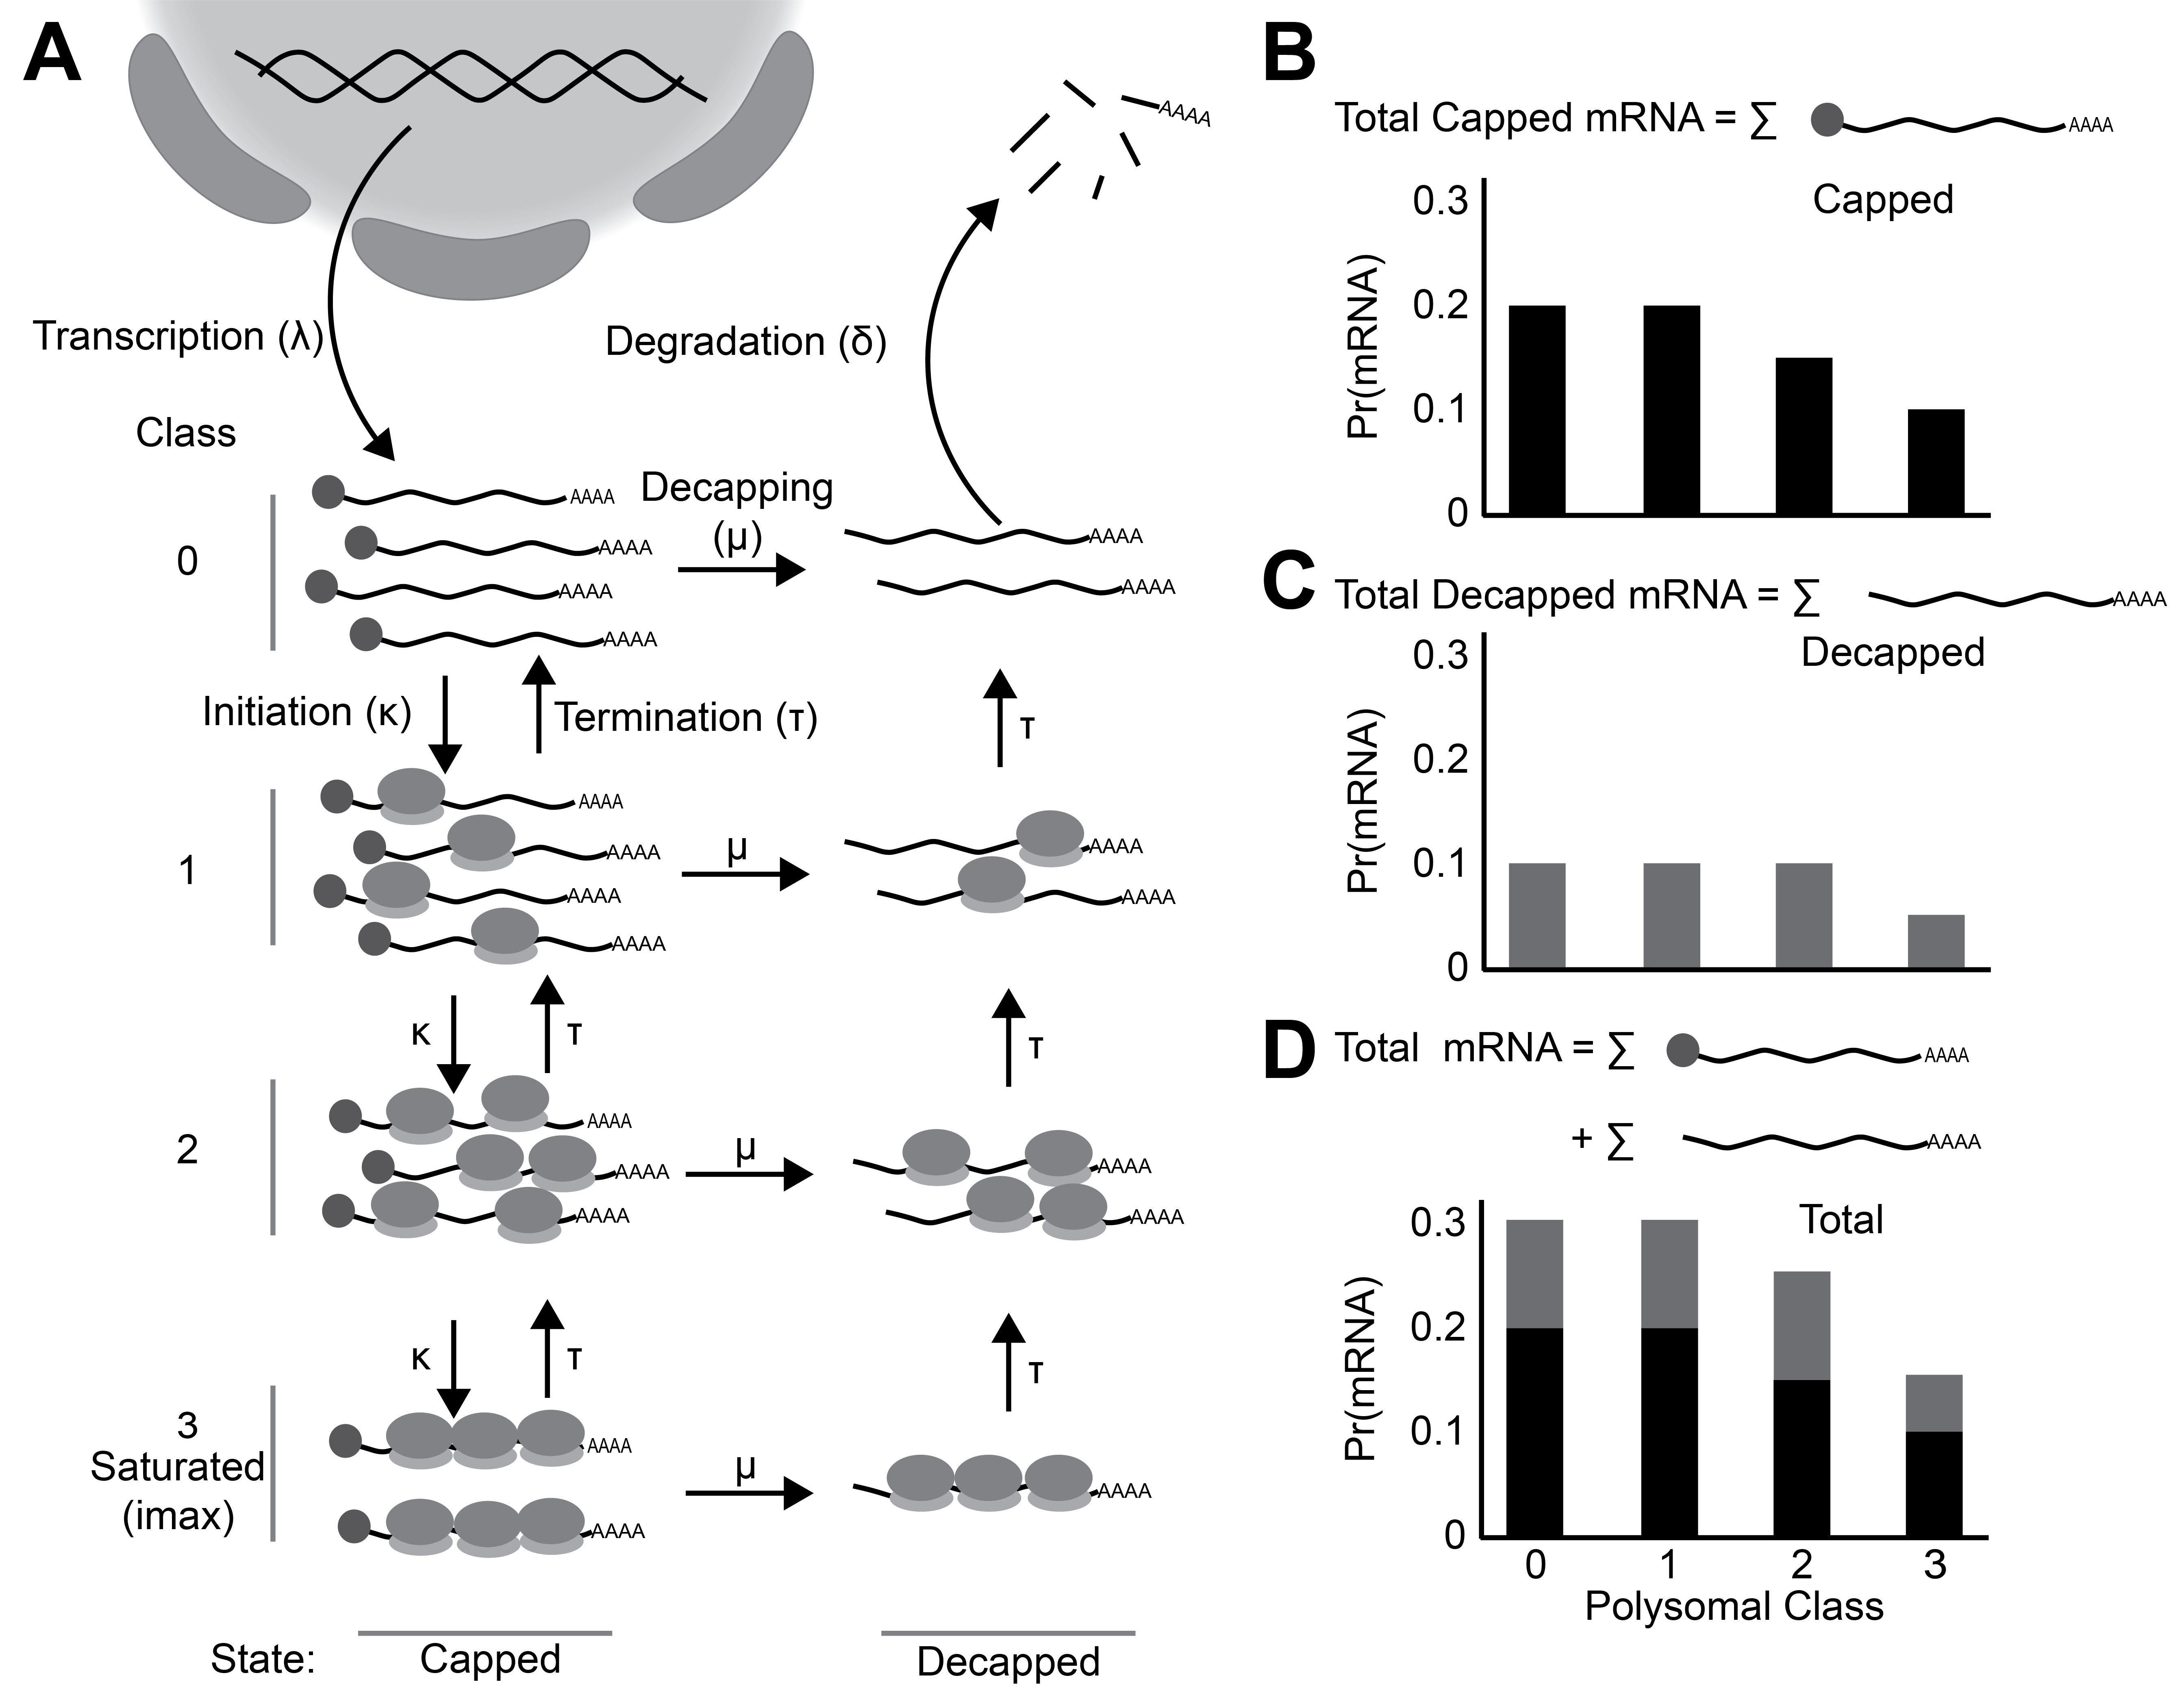
\includegraphics[width=120mm]{Images/Figure1_biomodel_V3.png}
\caption{{\bf Cartoon Representation of model in biological context.} 
{\bf A)} Model overview. Transcripts enter the sytem into the capped state at class 0 (no ribosomes bound). They enter the state at rate $\lambda$ through transcription. Transcripts are free to move up and down polysome classes at rates $\kappa$ for translation initiation and $\tau$ for elongation/termination. Transcripts can also be decapped and enter the decapped state at rate $\mu$. Finally, upon reaching class 0 in the decapped state transcripts are fully degraded at rate $\delta$. {\bf B)} Probability of finding an mRNA in each class in the capped state. {\bf C)} probability of finding an mRNA in each class in the decapped state. {\bf D)} Joint probabilty of finding an mRNA in each class across each state. This reflects the total protein production potential.}
\label{fig1}
\end{center}
\end{figure}
%\clearpage


Transcripts enter into the model as defined by the transcription rate $\lambda$ into the capped state with no ribosomes,  ie. polysome class 0 ($m_0$). 
From the $m_0$ class a transcript can have two fates. 
The transcript can be decapped, thus marked for degradation at rate $\mu$ and move into the decapped class $m_0*$.
Alternatively, a ribosome can initiate translation on the mRNAs in the capped, ribosome free polysome class 0 at rate $\kappa$ and be loaded onto the transcript and move it into capped class $m_1$.
Because only one ribosomes can occupy a particular location on the mRNA at any given time, and our model does not track ribosomal positions, we model translation intiation across polysome classes $i = 0$ to $\imax$, more generally as
\begin{equation}
  \label{eq:kappa_i}
  \kappa_i = \kappa_0 \left(1- \frac{i}{\imax}\right),
\end{equation}
where $i$ is the mRNA polysome class, \imax is the maximal ribosomal occupancy on the transcript.
We note $i/\imax$ represents, under the assumptions of a uniform distribution,  the probability a randomly chosen codon position is occupied by a ribosome.
Correspondingly, $1 - i/\imax$ represents probability a randomly chosen codon position, such as the initiation site is unoccupied.
Because the natural units for mRNA coding sequence length in our model is the amount of space the bound ribosome takes when translating it follows that $\imax = n_{c}/9$ where $n_{c}$ is the length of the mRNA's coding sequence in codons and 9 represents the length in codons of space a single ribosome occupies.
%$\imax = n_{\text{nt}}/27$ where $n_{\text{nt}}$ is the length of the mRNA's coding sequence in nucleotides.
This attempts to account for the ribosomal density dependent effects on initiation and is called the density dependent initiation (DDI) model.


A ribosome on the transcript elongates the peptide and, in turn, terminates at a rate of $\tau$, 
Given that the length scale of our model is formulated in terms of ribosome widths but most estimates of elongation are at the scale of codons, if $\tau_c$ is the average elongation rate of an mRNA in codons, $\tau = \tau_c/9$.
As the number of ribosomes on a transcript increase, the probability of a ribosome being at the end of the transcript also increases.
Again assuming ribosomes are distributed across a transcript according to a uniform distribution, the expected ribosome termination rate on a mRNA in polysome class $i$ is simply, 
\begin{equation}
	\tau_i = \tau \frac{i}{\imax}.
\end{equation}


Capped transcripts move through rounds of translation initiation and elongation-termination and are distributed along the different polysomal classes. 
From any polysome class in the capped state $m_i$ the transcript can be decapped at rate $\mu$  and move into the decapped state while maintaining the same polysomal class $m_i^*$.
Decapped transcripts can no longer initiate new rounds of translation, but allow for currently loaded ribosomes to complete translation. 
The behavior of the $m_i^*$ classes represent co-translational decay, a common method of mRNA decay in eukaryotes~\cite{RN3,RN23,RN4}. 
After all ribosomes on a decapped transcript complete translation, the mRNA is in decapped class 0 and completely degraded at the mRNA clearance rate $\delta$.

The model produces two outputs. 
First, the total mRNA in either the capped or decapped state and therefore the system (Fig \ref{fig1}B-D). 
Second, the distribution of the mRNAs in each mRNA in each polysome class. (Fig \ref{fig1}B-D).

We represent each state by a series of coupled ordinary differential equations (ODEs), one equation for the mRNA population for each polysome class. 

The functional form of the capped mRNA sub population is:
%\pagebreak 

%\begin{table*}
%\caption{Derivation of Result XYZ}
%\centering
%\begin{minipage}{0.75\textwidth}

\begin{strip}
\begin{align} \label{eq:Capped_ODE}
\frac{dm_{0}}{dt} &= \lambda+ \tau \frac{1}{\imax}m_{1}-\left(\kappa_0 + \mu\right)m_{0} \nonumber \\
\frac{dm_{1}}{dt} &= \kappa_0 m_{0}+ \tau \frac{2}{\imax}m_{2}-\left( \tau \frac{1}{\imax}+\kappa_0\left(1-\frac{1}{\imax}\right)+\mu\right) m_{1}\nonumber \\
& \vdots & \nonumber \\
\frac{dm_{i}}{dt} &= \kappa0 \left(\frac{i-1}{\imax}\right) m_{i-1}+ \tau \frac{i+1}{\imax}m_{i+1}-\left( \tau \frac{i}{\imax}+\kappa_0\left(1-\frac{i}{\imax}\right)+\mu\right) m_{i} \nonumber \\
& \vdots & \nonumber \\
\frac{dm_{\imax}}{dt} &= \kappa_0\left(1-\frac{\imax-1}{\imax}\right)m_{\imax-1}-\left( \tau +\mu\right) m_{\imax}
\end{align}
\end{strip}

Similarly, the functional form of the decapped mRNA sub population is: 
\begin{align}\label{eq:Decapped_ODE}
\frac{dm_{0}^{*}}{dt} &= \mu m_{0}+ \tau \frac{1}{\imax}m_{1}^{*}-\delta m_{0}^{*} \nonumber \\
\frac{dm_{1}^{*}}{dt} &= \mu m_{1}+ \tau \frac{2}{\imax}m_{2}^{*}-\tau \frac{1}{\imax} m_{1}^{*} \nonumber \\
& \vdots & \nonumber \\
\frac{dm_{i}^{*}}{dt} &= \mu m_{i}+ \tau \frac{i+1}{\imax}m_{i+1}^{*}-\tau \frac{i}{\imax} m_{i}^{*} \nonumber \\
& \vdots & \nonumber \\
\frac{dm_{\imax}^{*}}{dt} &= \mu m_{\imax}^{*}- \tau m_{\imax}. 
\end{align}

In closing, we note the parameters $\imax, \kappa, \mu,$ and $\tau$ likely vary between genes.


\begin{table}[!ht]
\begin{adjustwidth}{-2.25in}{0in} 
\centering
\caption{{\bf State variables and model parameters for ODE model of mRNA populations.}}
\begin{tabular}{|rp{4in}|c|c|c|}
\hline
\textbf{Symbol}&\textbf{Description}&\textbf{Unit} \\\hline
State Variables & &  \\ 
\hline
$m_i$ & Abundance of mRNAs with a ribosome load of $i$ in capped state. & $mRNA$ \\
$m_i^*$ & Abundance of mRNAs with a ribosome load of $i$ in decapped state. & $mRNA$ \\ \hline
$p_i$ & Probability of finding an mRNA with a ribosome load of $i$ in capped state. & \\
$p_i^*$ & Probability of finding an mRNA with a ribosome load of $i$ in decapped state. &  \\ \hline
\multicolumn{1}{l}{Model Parameters} \\ \hline
$i$ & ribosomal load index & Ribosome\\
 \imax & Maximum number of ribosomes able to bind to mRNA\\ & Ribosome \\
$\kappa_0$ & Translation initiation rate for capped mRNAs with a ribosome load of $i=0$. & $1/s$\\
$\tau$ & Translation completion rate for one ribosome & $1/s$\\
$\mu $ & Decapping rate. & $1/s$\\
$\lambda$ & Production rate of newly produced, ribosome free, and capped mRNA to the $m_0$ class. & $mRNA/s$\\
$\delta$ & Removal rate of decapped mRNA with a ribosome load of 0 from the $m_0^*$ class. & $1/s$\\ \hline 
\multicolumn{3}{|p{450pt}|}{\footnotesize Note: $\mathbb{R}^+$ represents the non-negative real numbers and $\mathbb{Z}^{(+)}$ represents the strictly positive integers.} \\ \hline
\end{tabular}
\begin{flushleft}
Variable \imax is in the domain of non-negative integers; all other variables are non-negative real numbers.
The mRNA unit is the number of molecules of mRNA.
\end{flushleft}
\label{tab:params}
\end{adjustwidth}
\end{table}


\subsubsection*{Steady state solutions of the capped transcript population}
 The model solution for the capped state can be represented in the following form,
	\begin{equation} \label{eq:capped_solution}
		\mvechat=\frac{\lambda}{\mu}\vec{p}_m
	\end{equation}

Where \mvechat is a vector of the steady state mRNA abundances in each polysomal class.
\mvechat is calculated from by scaling  the vector $\vec{p}$ (where $\sum \vec(p) = 1$), which represents the steady state distribution of the mRNA across the polysomal classes, by transcript production rate $\lambda$ and the decapping rate $\mu$.
While the individual components of $\vec{p}$ are functions of $i$, \imax, the translation initiation rate $\kappa$, the elongation rate $\tau$ and $\mu$, we could not find a closed form solution.
Regardless, it follows that the total abundance of the capped class \msum is,
\begin{equation}\label{eq:capped_sum}
\msum = \sum_{i = 0} ^\imax m_i = \lambda/\mu
\end{equation}

\subsubsection*{Steady state solutions of the decapped transcript population}

The solution for the decapped system is dependent on the underlying distribution of the capped system and can be represented as:

\begin{align} 
\label{eq:decapped_abundance}
\mhatstar_0  &= \frac{\mu}{\delta}\sum_{j=0}^{\imax}m_{j} \nonumber \\
\mhatstar_1  &= \frac{\mu}{\tau}\sum_{j=1}^{\imax}m_{j}  \nonumber \\
& \vdots &  \\
\mhatstar_i  &= \frac{1}{i}\frac{\mu}{\tau}\sum_{j=i}^{\imax}m_{j}  \nonumber \\
& \vdots & \nonumber \\
\mhatstar_{\imax}  &= \frac{1}{\imax}\frac{\mu}{\tau} \mvechat_{\imax}   \nonumber
\end{align}

We can simplify the model by converting the mRNA quantity $m_{j}$ to the probability $p_{j}$ by Eq (\ref{eq:capped_solution}). By defining $S_{j}$ as the cumulative probability from an mRNA found in class $i$ and above as,
\begin{equation}
		S_{i} = \sum_{i}^{\imax}\vec{p_{i}}
\end{equation}

Now the solution to Eq (\ref{eq:decapped_abundance}) becomes,

\begin{align}
\label{eq:decapped_solution} 
\mhatstar_0  &= \frac{\lambda}{\delta}S_{0}=\frac{\lambda}{\delta} \nonumber \\
\mhatstar_1  &= \frac{\lambda}{\tau}S_{1} \nonumber \\
& \vdots &  \\
\mhatstar_i  &= \frac{1}{i}\frac{\lambda}{\tau}S_{i}  \nonumber \\
& \vdots & \nonumber \\
\mhatstar_{\imax}  &= \frac{1}{\imax}\frac{\lambda}{\tau}S_{\imax}  \nonumber
\end{align}
 Note that $S_{0}=1$ and $ S_{0} \ge ... \ge S_{i} \ge ... \ge S_{\imax}$ highlighting the fact that the steady state solution for the decapped state \mvecstar is dependant on the distribution of mRNA polysome classes of the capped state the solution of the cumulative distribution function $S_i$. %The pattern of  the  $S$ means that $m_0 \ge m_1 \ge ... \ge ... m_i \ge ... \ge m_imax$.

The total transcript population in the decapped state $\mhatstar_{tot}$ does not have a closed form solution. However it can be summarized as follows,


\begin{align*}
	\msumstar = \sum_{i=0}^{\imax} m_{i}^{*} = \frac{\lambda}{\delta} + \frac{\lambda}{\tau}S_{1}+ \hdots \\
 + \frac{\lambda}{i \tau}S_{i} + \hdots  + \frac{\lambda}{\imax \tau}S_{\imax} 
\end{align*}

This can be further shortened to:
\begin{equation} \label{eq: marked_total_pop}
	\msumstar = \lambda(\frac{1}{\delta} + \frac{1}{\tau}\vec{S} \cdot \vec{l}	) 
\end{equation}
Where $\vec{S}$ is a vector of all the cumulative sums and $\vec{l}$ is a vector of $1,\frac{1}{2},...,\frac{1}{\imax}$ . 


To get the probability distribution of transcripts across the decapped state we can divide $\vec{m^{*}}/\msumstar$ which results in,
\begin{align}\label{eq:decapped_distribution}
	p_{0}^{*} &= \frac{1}{1 + \frac{\delta}{\tau}\vec{S} \cdot \vec{l}}	\\
  	p_{i}^{*} &= \frac{S_{i}}{i(\frac{\tau}{\delta} + \vec{S} \cdot \vec{l})}	\:\:\:\: \text{for } i=1, 2, ..., \imax
\end{align}

\subsubsection*{Calculation of the total mRNA population and its distribution between capped and decapped states}
Drawing on the definitions above, the total abundance of capped and decapped mRNA polysome classes ($\msumtot$) is defined by,
\begin{equation}
	\msumtot = \msum + \msumstar = \frac{\lambda}{\mu} +  \lambda(\frac{1}{\delta} + \frac{1}{\tau}\vec{S} \cdot \vec{l})
\end{equation}

To understand how mRNA is divided  between we start with the probability of finding an mRNA in the capped state.
\begin{equation*}
	\mfrac = \frac{1}{(1  + \frac{\mu}{\delta} + \frac{\mu}{\tau}\vec{S} \cdot \vec{l})}	
\end{equation*}
Then we calculate the odds,
\begin{equation}\label{eq:odds}
	odds_{\hat{m}} = \frac{1}{\mu(\frac{1}{\delta} + \frac{1}{\tau}\vec{S} \cdot \vec{l})} 
\end{equation}

\subsubsection*{Calculating expected ribosomal load and protein production}
The expected ribosomal load for the capped or decapped state calculated, respectively, by,
\begin{align}\label{eq:Expected_ribo_load}
  \MRL =& E_{\mvec}\left(\ribosome\right) =\sum_{i=0}^{\imax}i \times p_{i}  \\
   \intertext{and} \nonumber
   \MRL^* =& E_{\mvecstar}\left(\ribosome\right) =\sum_{i=0}^{\imax}i \times p^*_{i}\nonumber
\end{align}
Thus, the global mean ribosomal load is,

\begin{align} \label{eq:System_ribo_load}
	\text{Total Ribosomal Load} = \mfrac\times E_{\msum} \left(\ribosome\right) + \\
          + (1-\mfrac)\times E_{\msumstar}\left(\ribosome\right) \nonumber \\
\end{align}


%The maximum possible ribosomal load for our model is:
%\begin{equation}\label{eq:Max_output}
%	\text{Max output} = \lambda (\frac{1}{\mu}(\imax\tau) + (\frac{1}{\delta} + \frac{1}{\tau}H_{\imax}) (\frac{\imax}{(\frac{\tau}{\delta}+H_{\imax}) }\tau) )
%\end{equation}
%
%Where $H_{\imax}$ is the harmonic number for \imax.
\subsection*{Numerical solution implementation in R}
Code to solve the model was written and is freely available as an R package at (\url{https://github.com/rurquidi/Ribosome}). To solve the capped subsystem of the model, the \texttt{solve.tridiag} function from \texttt{limSolve package} (v1.5.6)~\cite{RN41}. The decapped solution was obtained by using the capped solutions into eq. (\ref{eq:decapped_solution}). Utility functions, plots and statistics were created using  \texttt{R} (v 3.6)~\cite{RN43}, and  \texttt{data.table} (v1.14.0)~\cite{RN42}. 
		
\subsection*{Data Sources}

In order to biologically contextualize and illustrate our model's behavior, we use on parameter values derived from the literature.
Protein lengths were extracted from the Ensembl (version 109) and Ensembl plants (version 56) respectively~\cite{RN26,RN25,RN24}.  
The range of \imax is determined from the distribution of protein lengths obtained from brewer's yeast (\textit{saccharomyces cerevisiae}) and \textit{Arabidopsis thaliana}. The range of \imax is  48 (36) (mean (SD)) for yeast and 47 (30) for Arabidopsis (Fig \ref{fig2}A and C).
The decapping rate between the capped and uncapped system was estimated from the protein half-lives from Presnyak (2015) for yeast (Fig \ref{fig2}B) and Sorenson (2018) for Arabidopsis (Fig \ref{fig2}D)~\cite{RN27,RN28}.
We estimated gene specific $\mu$ from the half lives with the following:
	\begin{equation*}
		\mu_i = \frac{\ln(2)}{t_{1/2_i}}
	\end{equation*}

Where $t_{1/2}$ is the half-life. The resulting range of $\mu$ is from $1.3 \times 10^-3 (1.8 \times 10^-3)$ for yeast and $1.7 \times (10^-4 \pm 2 \times 10^-4)$ for Arabidopsis. 

\begin{figure*}[!h]
\begin{center}
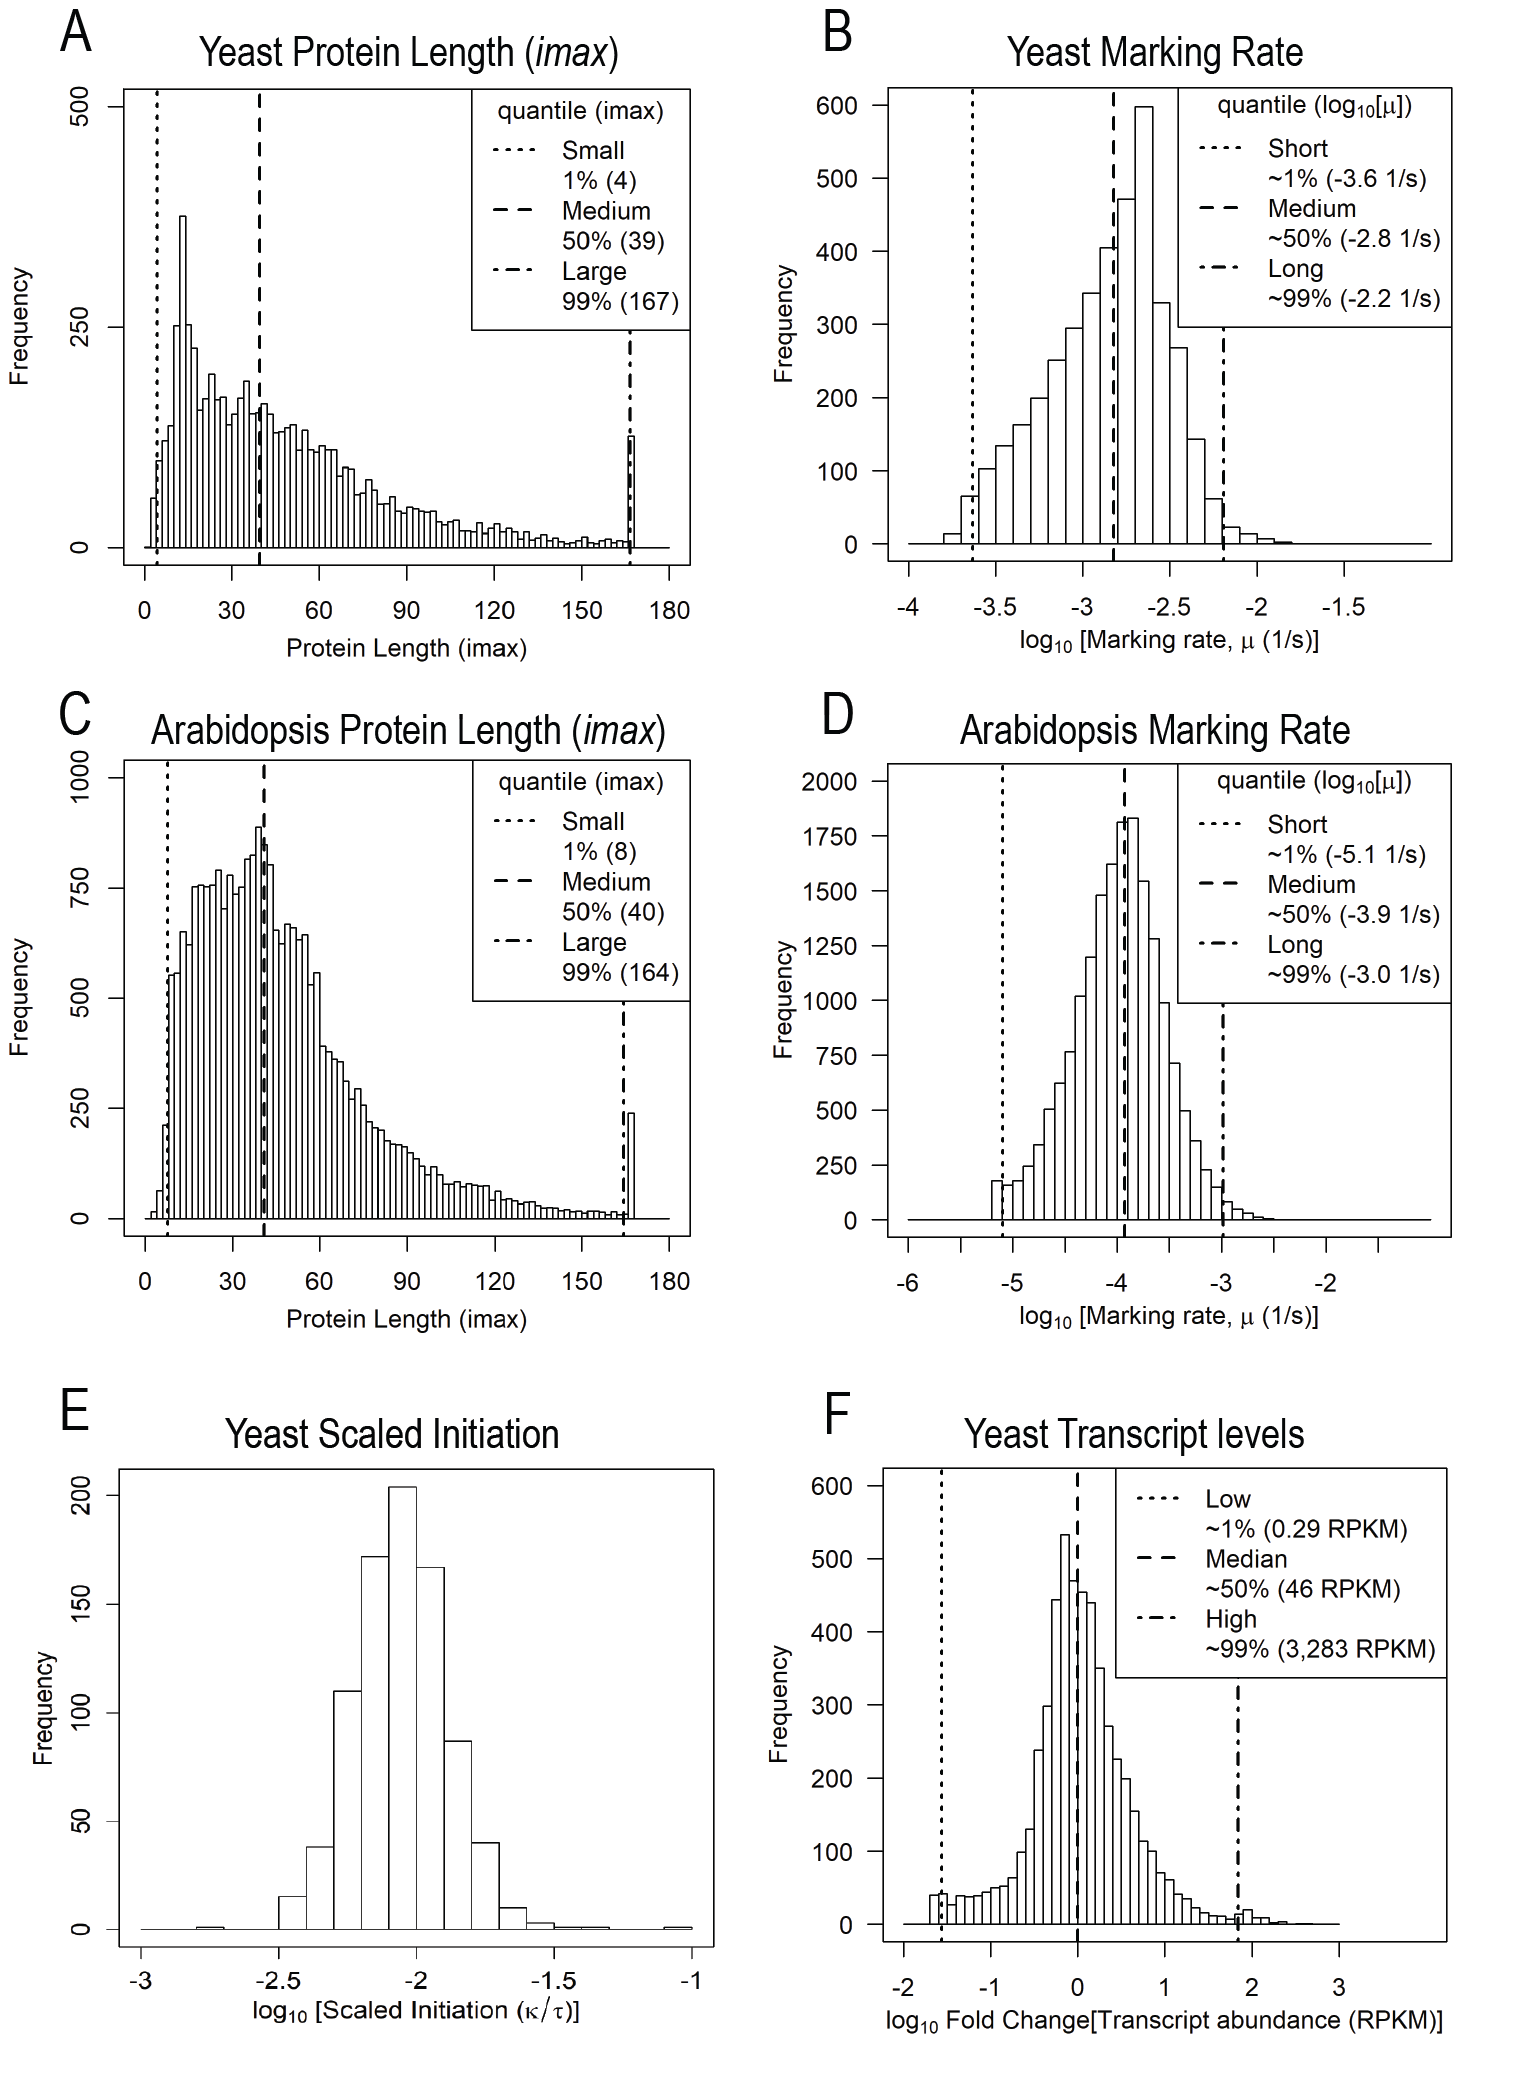
\includegraphics[width=120mm]{Images/2023-07-04_parameter_histograms.png}
\caption{{\bf Histograms of empirical values of model parameters.}
{\bf A)} Yeast protein lengths. {\bf B)} Yeast half-life {\bf C)} Arabidopsis Protein Lengths. {\bf D)} Arabidopsis Half-Life. {\bf E)} Yeast Scaled elongation rates (Translational initiation rate/average translation elongation rate) on a per gene basis. {\bf F)} Log 10 Fold Changes between all transcripts compared ot the median transcript expression in yeast. }
%\centering Red: de_s class, Green: capped class, Blue: Total= capped+decapped classes}
\label{fig2}
\end{center}
\end{figure*}


Translation initiation and average elongation rates ($\kappa$ and $\tau_c$) were obtained for Yeast from Duc and Song 2018~\cite{RN13}. 
%In Duc and Song 2018, the authors used 850 highly translated transcripts from the ribo-seq dataset from Weinberg 2016. They employed a TASEP model to estimate the initiation rates and correct the empirical elongation rates from the footprint distributions. 
We calculated an average gene specific elongation rate from the corrected elongations rates. We scale the each gene specific initiation rate by dividing it by the gene specific elongation rate.
\begin{equation}
	\text{initiation to elongation ratio} = \kappa' = \frac{\kappa}{\tau}
\end{equation}

This simplifies the model behavior to one generalized parameter with a unique response (Fig \ref{fig2}E).  The initiation to elongation ratio ranges from 0.1$s^{-1}$ to 0.001$s^{-1}$.

The transcriptomic results from Weinberg 2016 are included in Fig \ref{fig2}F. In short, reads per kilobase million from Weinberg were further converted into a log10 fold change based on the median expression level~\cite{RN29}. Fig \ref{fig2}F shows that the absolute range of transcriptional expression ranges just under 5 orders of magnitude. Because transcription rate $\lambda$ acts as a scaling factor throughout the model and does not affect the distribution of the ribosomes, for simplicity we set $\lambda$ = 1.

Because the mRNA clearance rate $\delta$ only determines the accumulation of transcripts in the  $m_0^*$  class, for simplicity, we set $\delta >> \tau$ and thus  $m_0^* \sim 0$.
 
The empirical mean ribosomal load (\MRL) for the 850 genes in Duc and song 2018 was calculated from the mRNA-seq read per kilbase million (mRNA RPKM) and the ribo-seq footprints (RPF RPKM) from Weinberg 2016~\cite{RN29}. The following equation was used.
\begin{equation}\label{eq:MRL}
	\MRL_i = \frac{\text{RPF} \: \text{RPKM}_i}{\text{mRNA} \:  \text{RPKM}_i  \times \frac{200}{\text{length mRNA}_i}}
\end{equation}

Where the gene specific scaling factor $\frac{200}{\text{length mRNA}_i}$ corrects for the bias in read counts due to longer transcripts producing more fragments. The value 200 arises from the average fragment size of a library prep and can be adjusted according the experimental method used.



% It could be futher extended to include more degradations mechanisms see note below
% $\delta\ might be more complex with a slightly different model design. In the current model formulation it mimics the primary (but not only) degradation with the cell, the 5' decapping and subsequent VCS /XRN1 5'-3' cotranslation degradation system. This ignores 3 other systems the two 3'- 5' pathways (CCR4-NOT3) and exosome, and the final slew of endodegradation pathways (NGD, NSD, NMD, ribothrypsis, and silencing).
%Additionally, degradation of the bulk of the mRNA transcript might not be a process specific to each transcript (ie. due to coding sequence, I would have to look this up. Also might be testable with data fitting).


\section*{Results}

\subsection*{Model presents steady state distribution of mRNAs across polysome classes for each initiation to elongation ratio}

The model predicts the abundances of the mRNA in the capped and decapped states as well as the mRNA's distribution across polysome classes.

\subsubsection*{Steady state distribution of the capped mRNA polysome classes}

The analytical steady state solution eq. (\ref{eq:capped_solution}) is composed of a vector of probabilities $\vec{p_m}$ that an mRNA is in polysome class $i$ and a scaling term (the transcription rate $\lambda$ divided by the decapping rate $\mu$). 
This solution highlights two separate roles of $\mu$. 
First, the scaling term $\lambda / \mu$ determines total mRNA abundance in the capped state. 
Second, the vector of probabilities is a function of the initiation rate $\kappa$, the elongation/termination rate $\tau$ and $\mu$ and is independent of $\lambda$.
Fig \ref{fig3}A shows the mRNA distribution in the capped state for four different initiation to elongation ratios $\kappa'$, for a protein of median length (\imax of 39) with a low decapping rate ($2\times10^{-4} /s$, 99\textsuperscript{th} percentile).
To summarize the model results across a range of parameters a heatmap where each row is the steady state distribution of mRNA at a particular $\kappa'$ is shown (Fig \ref{fig3}B).
The steady state density in the capped system is bounded at class 0 and class \imax 
When $\kappa'<<\tau$, the steady state distribution concentrates at low $i$ near the $i=0$ boundary.
As $\kappa'$ increases, the steady state distribution moves towards higher $i$ and can be roughly approximated by a truncated gaussian. 


\begin{figure}[!h]
\begin{center}
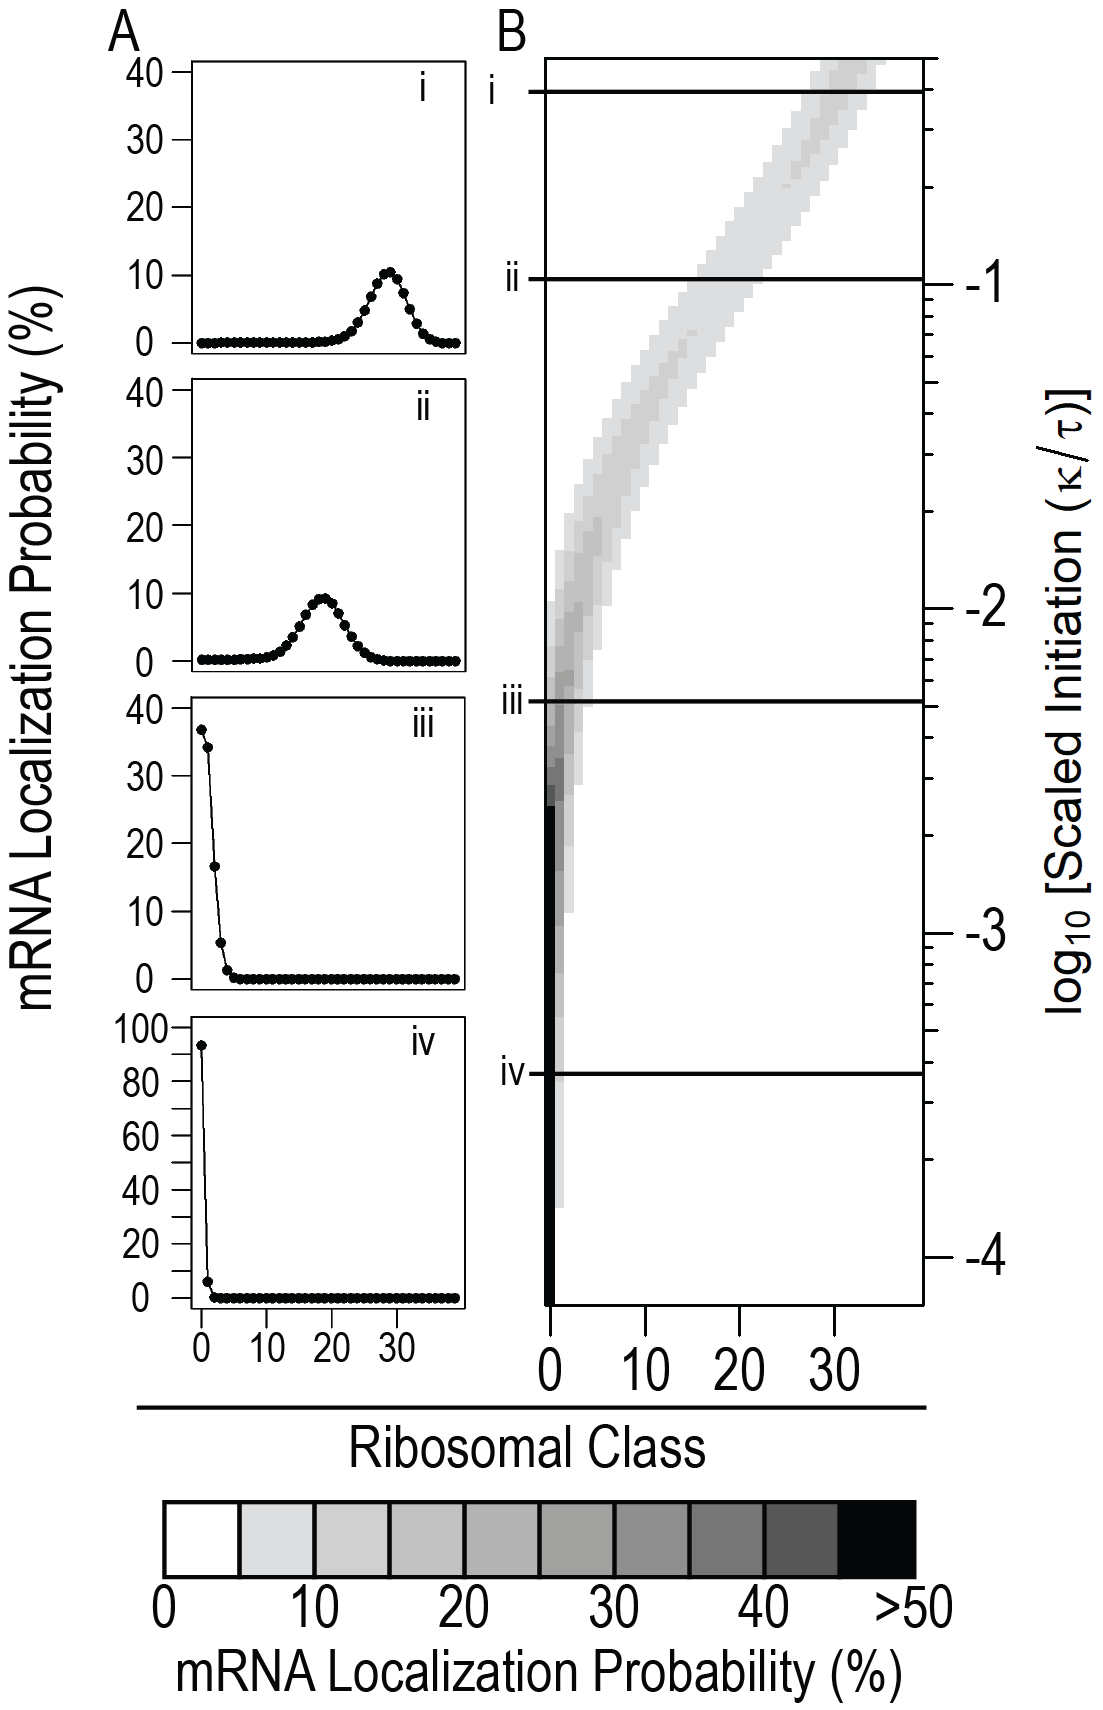
\includegraphics[width=75mm]{Images/2023-07-04_Unmarked_slices.png}
\caption{{\bf mRNA distribution in capped state.} {\bf A)} Distribution profiles for four scaled initiation values i) $2\times 10^{-1}$ ii) $1.03\times 10^{-1}$ iii) $3\times 10^{-3}$ iv) $2\times 10^{-4}$ {\bf B)} Heatmap of model output across a range of scaled initiation values. Lines represent slice represented in A). Results produced with \imax of 39 and a low decapping rate of $2\times10^{-4}$  (99\textsuperscript{th} percentile). Color bar shows probability of finding mRNA in a particular polysome class.}
%\centering Red: decapped class, Green: capped class, Blue: Total= capped+decapped classes}
\label{fig3}
\end{center}
\end{figure}


\subsubsection*{Steady state distribution of the decapped mRNA polysome classes}
The decapped state is again scaled by the transcription rate $\lambda$.
The analytical steady state solution eq. (\ref{eq:decapped_solution}) can be understood in two parts: $m_0^*$ and the remaining $m_i^*$ for $i>0$.
$m_0^*$ is solely determined by the ratio of the mRNA production rate to the clearance rate $\lambda / \delta$.
The remaining decapped polysome classes depend on the elongation/termination rate $\tau$ and the distribution of \mvechat.
 Fig \ref{fig4}A shows the mRNA distribution in the decapped state for $i>0$ under the same conditions as Fig \ref{fig3}, for a median length protein with a low decapping rate ($2\times10^{-4}$) and the full range of $\kappa'$ are shown in the heatmap in Fig \ref{fig4}B.
The mRNA distributions are greatest in the $i=1$ polysome class and are monotonically decreasing. 
 

\begin{figure}[!h]
\begin{center}
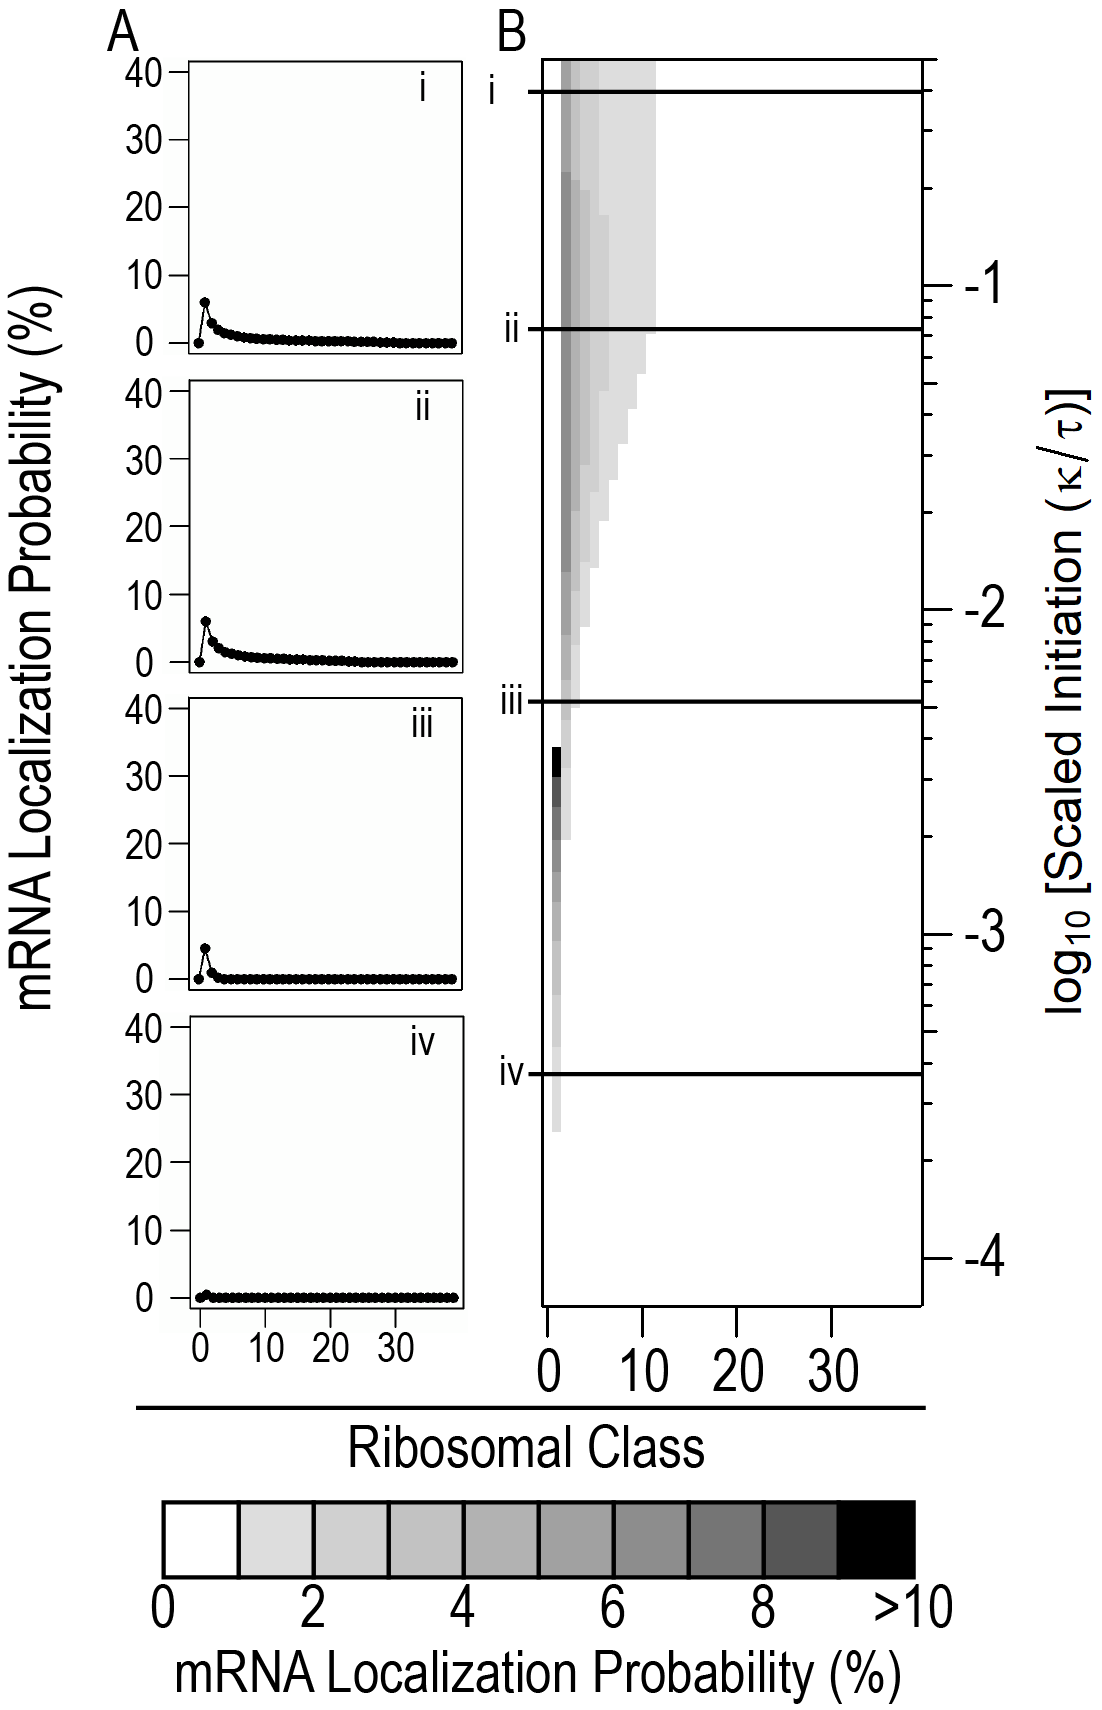
\includegraphics[width=75mm]{Images/2023-07-04_Marked_slices.png}
\caption{{\bf mRNA distribution in decapped state.}  {\bf A)} Distribution profiles for four scaled initiation values i) $2\times 10^{-1}$ ii) $1.03\times 10^{-1}$ iii) $3\times 10^{-3}$ iv) $2\times 10^{-4}$ {\bf B)} Heatmap of model output across a range of scaled initiation values. Lines represent slice represented in A). Results produced with \imax of 39 and a low decapping rate of $2\times10^{-4}$  (99\textsuperscript{th} percentile). Color bar shows probability of finding mRNA in a particular polysome class.}
%\centering Red: decapped class, Green: capped class, Blue: Total= capped+decapped classes}
\label{fig4}
\end{center}
\end{figure}


\subsubsection*{Steady state joint distribution for the combined capped and decapped mRNA classes}
The full model combines the mRNA distributions from the capped and decapped states, which is what is measured by most biological assays.
Fig \ref{fig5}A shows the mRNA distribution in the full model for three values of $\kappa'$, for a median length protein with a low decapping rate ($2\times10^{-4}$) and the full range of $\kappa'$ are shown in the heatmap in Fig \ref{fig5}B.
The system is unimodal at low $\kappa'<0.01$ when the capped and decapped distributions overlap around low $i$ (Fig \ref{fig5}A mid and low). 
As $\kappa'>0.01$ increases, the full distribution becomes bimodal (Fig \ref{fig5}A high).
The peak at low $i$ representing the decapped distribution, and the higher gaussian peak representing the capped distribution. 


\begin{figure}[!h]
\begin{center}
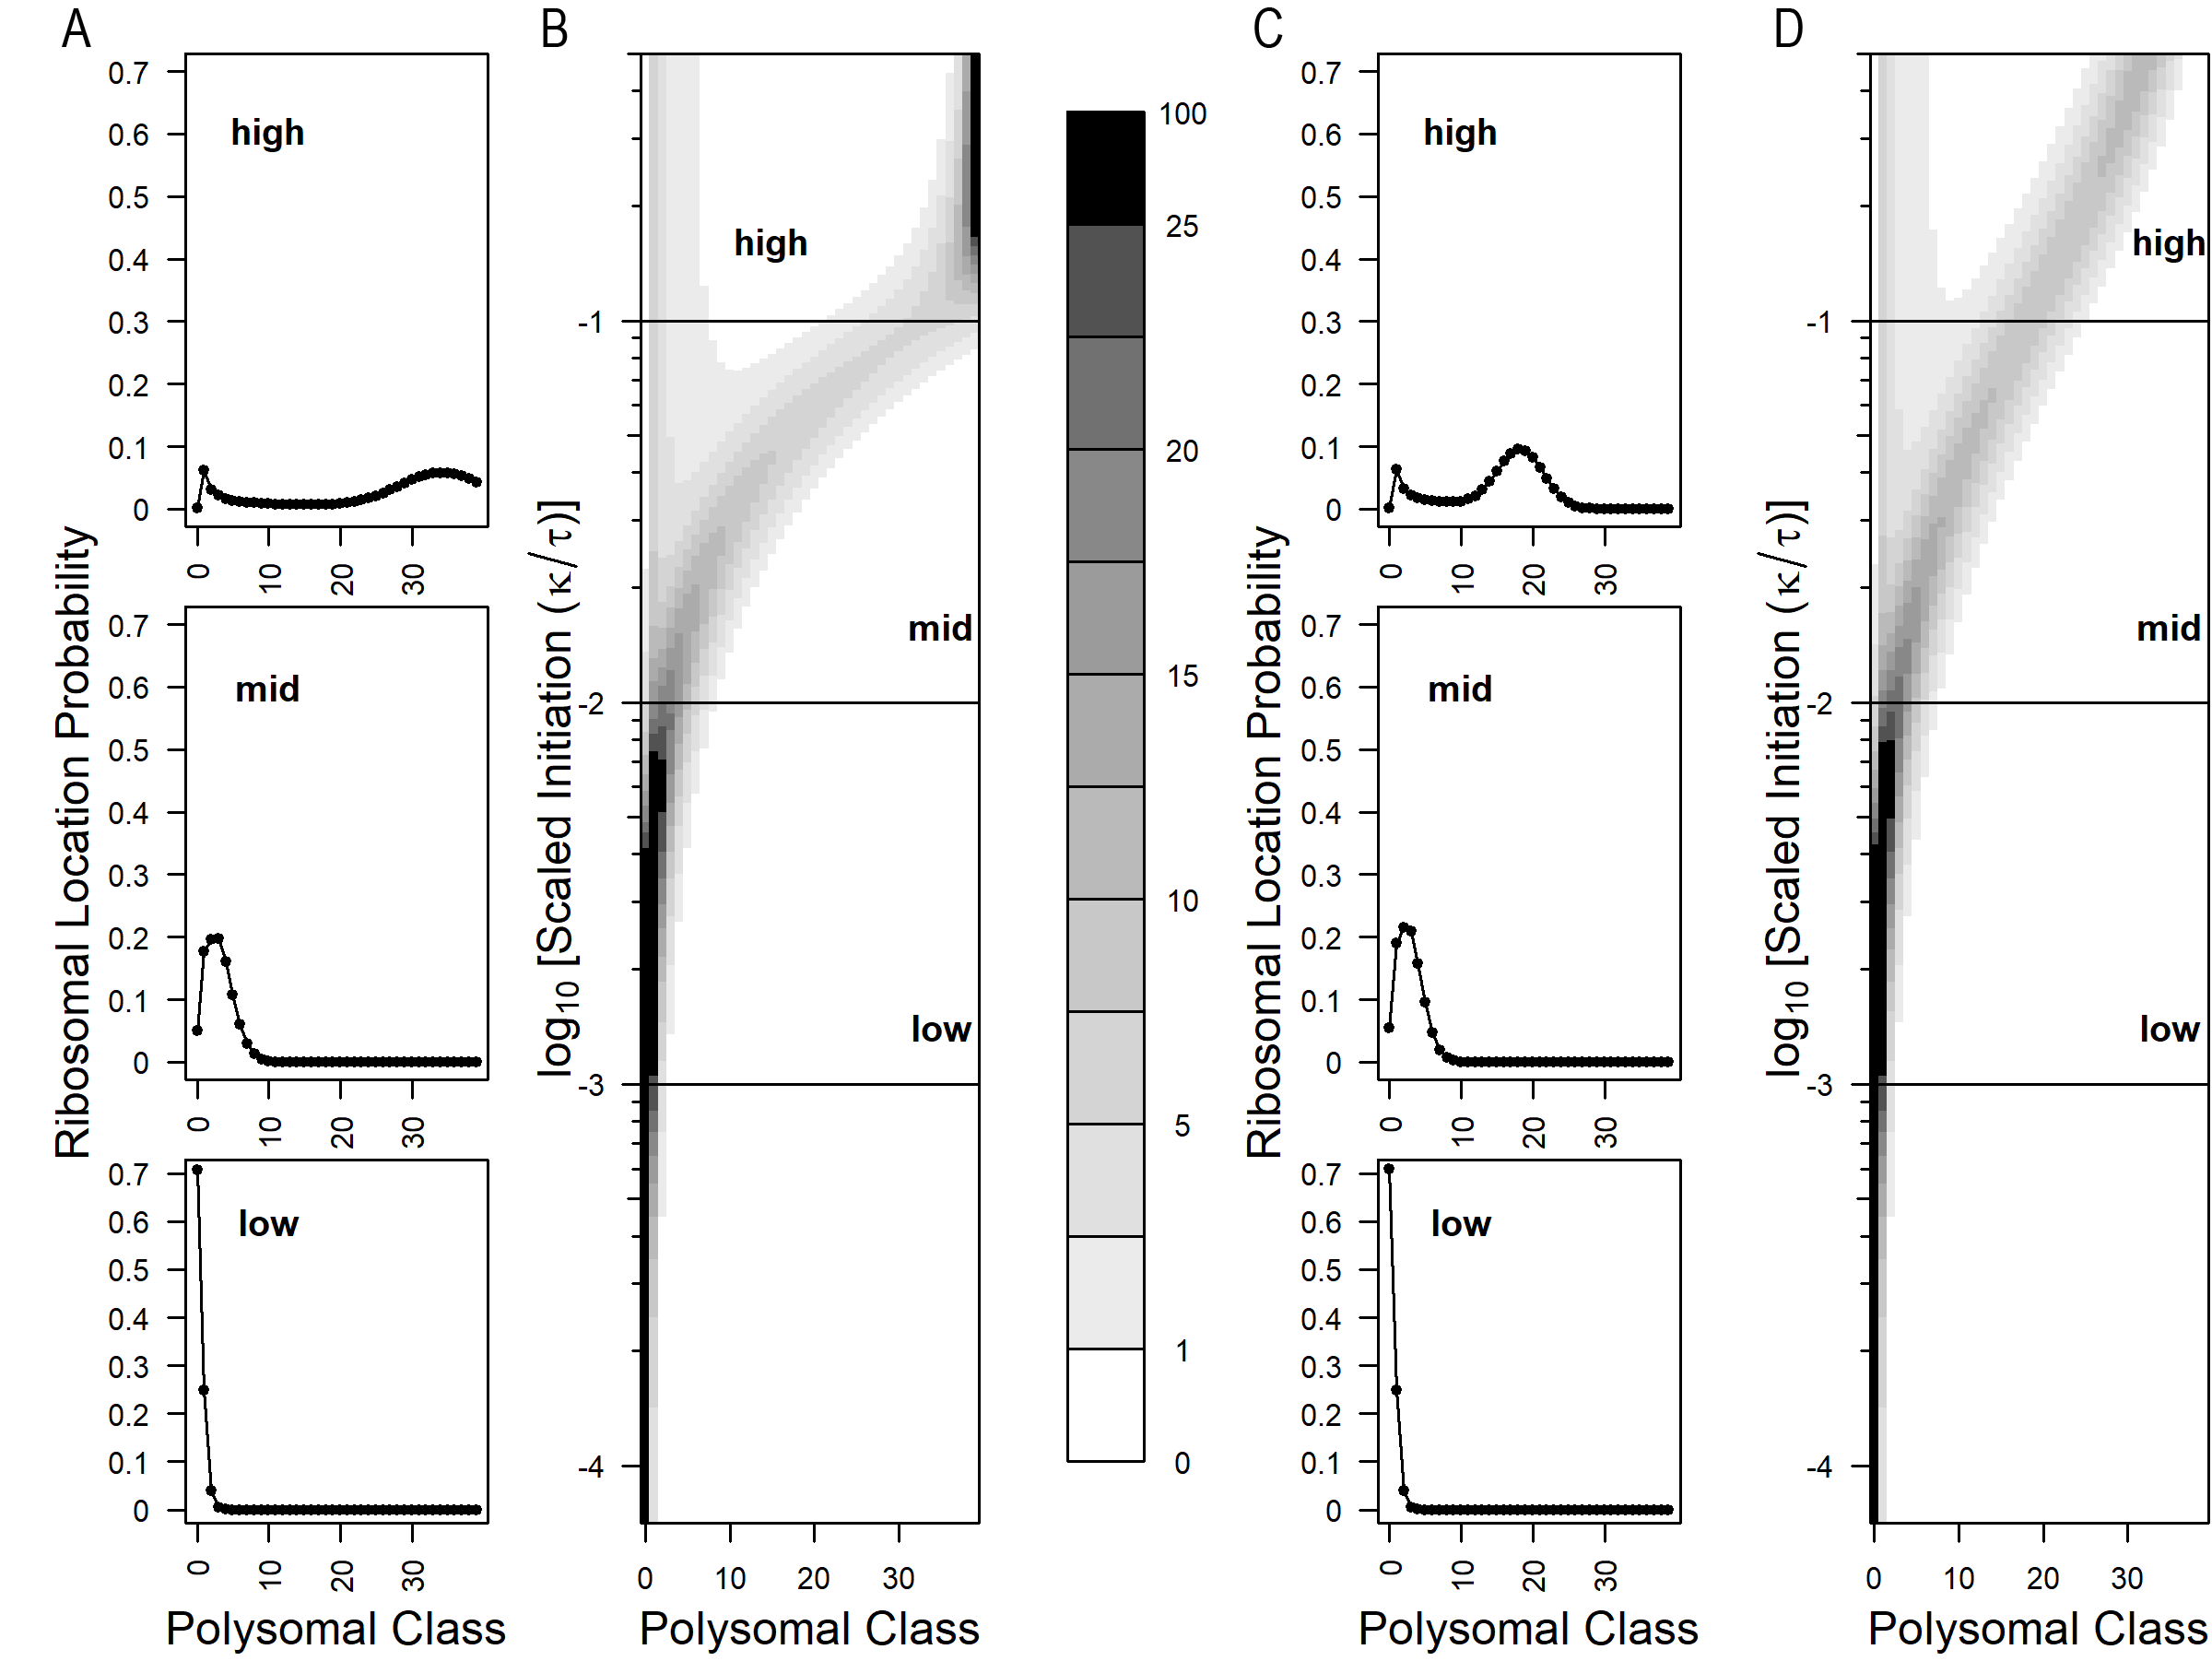
\includegraphics[width=75mm]{Images/2023-07-09_Figure1_DIIvsDDI_medianlength_low_marking_with_labels.png}
\caption{{\bf mRNA distribution in the full model.} {\bf A)} Distribution profiles for three scaled initiation values low) $1\times 10^{-3}$ mid) $2\times 10^{-2}$ and high) $1\times 10^{-1}$ {\bf B)} Heatmap of model output across a range of scaled initiation values. Lines represent slice represented in A). Results produced with \imax of 39 and a low decapping rate of $2\times10^{-4}$  (99\textsuperscript{th} percentile). Color bar shows probability of finding mRNA in a particular polysome class.}
%\centering Red: decapped class, Green: capped class, Blue: Total= capped+decapped classes}
\label{fig5}
\end{center}
\end{figure}


\subsection*{Decapping reduces ribosomal loads and shifts mRNA from the capped polysome classes to the decapped polysome classes}

To explore the role of mRNA stability on mRNA populations we varied the decapping rate $\mu$ from the 1\textsuperscript{st}, 50\textsuperscript{th} and 99\textsuperscript{th} percentile values as determined from ~\cite{RN27}.
As $\mu$ increases the distribution of mRNAs changes in two ways. 
First, there is shift to lower polysome classes in the capped state (Fig \ref{fig6}).
This is due to the mRNAs leaving the capped state at a higher rate and driving the equilibrium towards lower ribosomal loads. 
Secondly, as $\mu$ increases, a larger proportion of the mRNA is found in the decapped state. This is further explored later. 


\begin{figure*}[!h]
\begin{center}
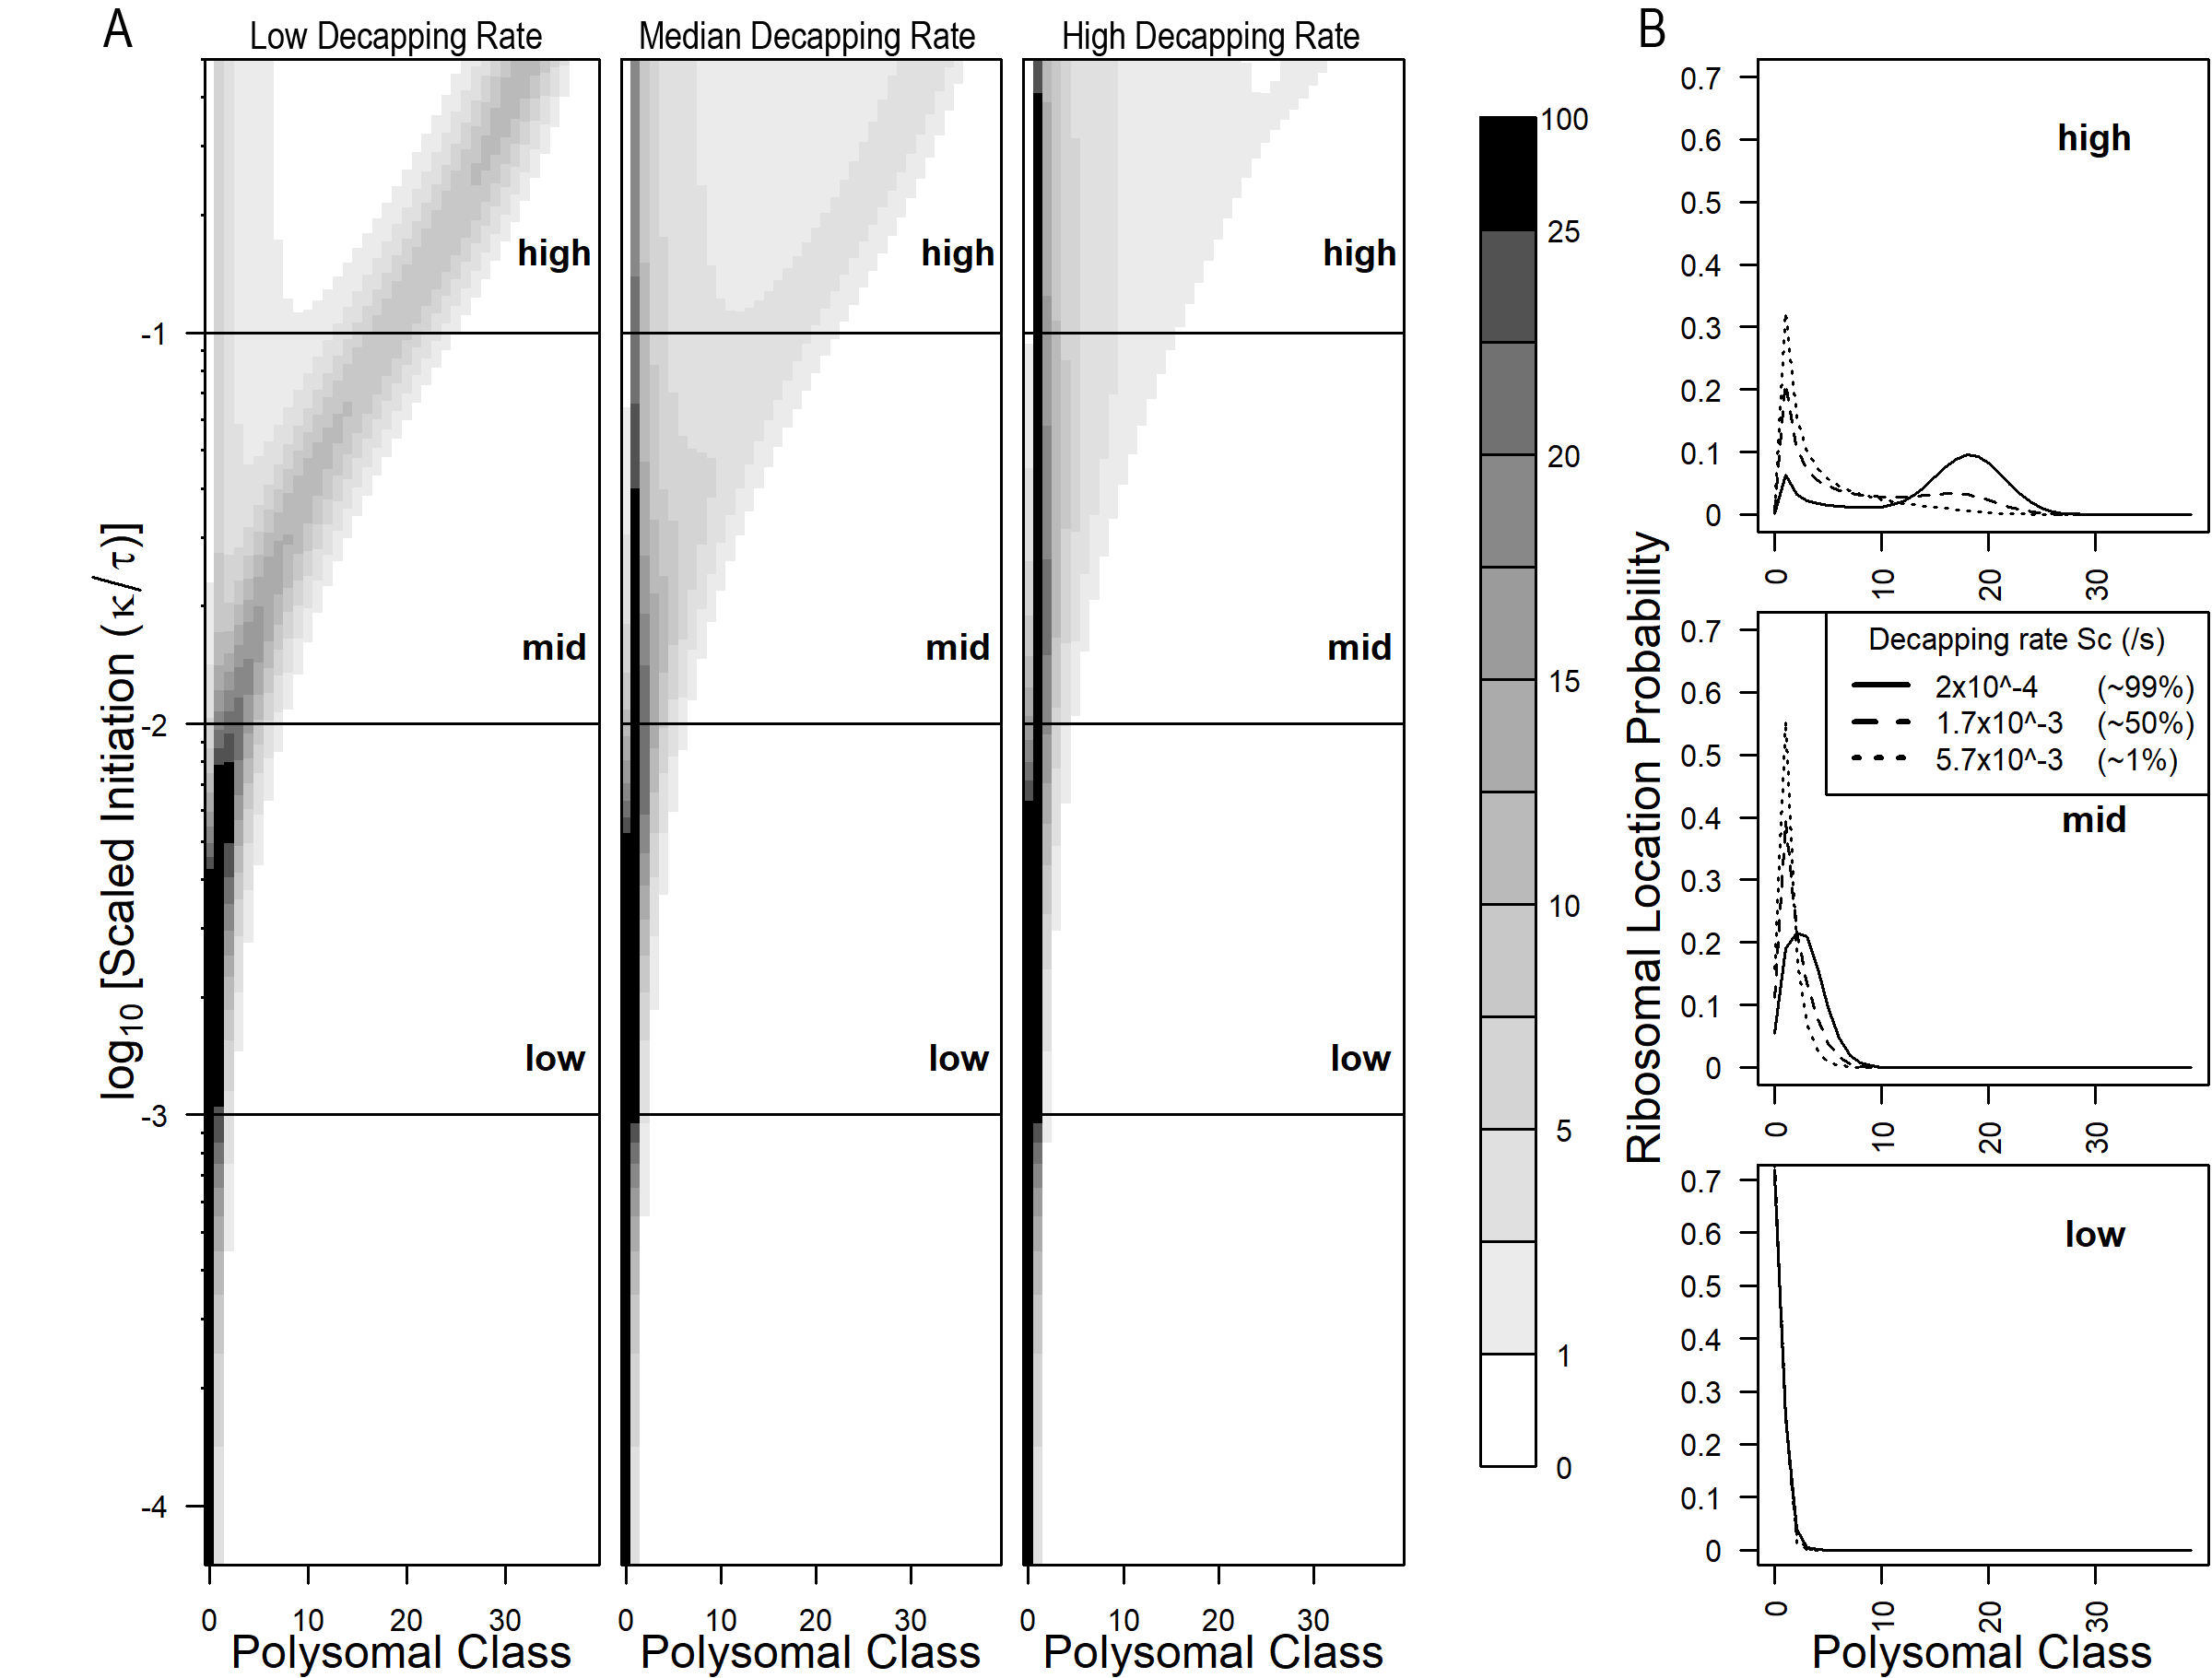
\includegraphics[width=140mm]{Images/2023-07-09_Figure2_Marking_Rate_range_medianlength_with_labels.png}
\caption{{\bf Higher decapping rates $\mu$ reduce ribosome load in the capped system in yeast.}  {\bf A)}  Heatmaps for the full model. Left) low $\mu$ ($2\times 10^{-4}$ /s) Center) median $\mu$ ($1.7\times 10^{-3}$ /s) Right) $\mu$ ($5.7\times 10^{-3}$ /s) {\bf  B)} individual density profiles for low (0.001), mid (0.01) and high (0.1) scaled initiation values for each $\mu$ All results calculate with \imax = 39.}
%\centering Red: decapped class, Green: capped class, Blue: Total= capped+decapped classes}
\label{fig6}
\end{center}
\end{figure*}


Plants and other multicellular eukaryotes tend to have lower translation initiation $\kappa$ and elongation rates $\tau$ as well as slower cell division when compared to single celled organisms such as yeast.
This is highlighted by the current gold standard study of mRNA half-lives in the model organism \textit{Arabidopsis thaliana}, where the estimated decapping rates $\mu$ estimated are ten to one hundred times lower than those in yeast. 
To explore the effect of lower $\mu$ in Arabidopsis (range: $7.7 \times 10^{-6}$ to $1 \times 10^{-3}$ ) vs yeast (range $2 \times 10^{-4}$ to $5.7 \times 10^{-3}$ ), we ran the model using the same initiation to elongation ratios as in yeast, the median Arabidopsis \imax of 41. 
As expected, the lower$\mu$ results in an mRNA distribution at higher $i$ (Fig \ref{fig7}) and are mostly in the capped polysome classes (Fig \ref{fig10}).


\begin{figure*}[!h]
\begin{center}
\centering
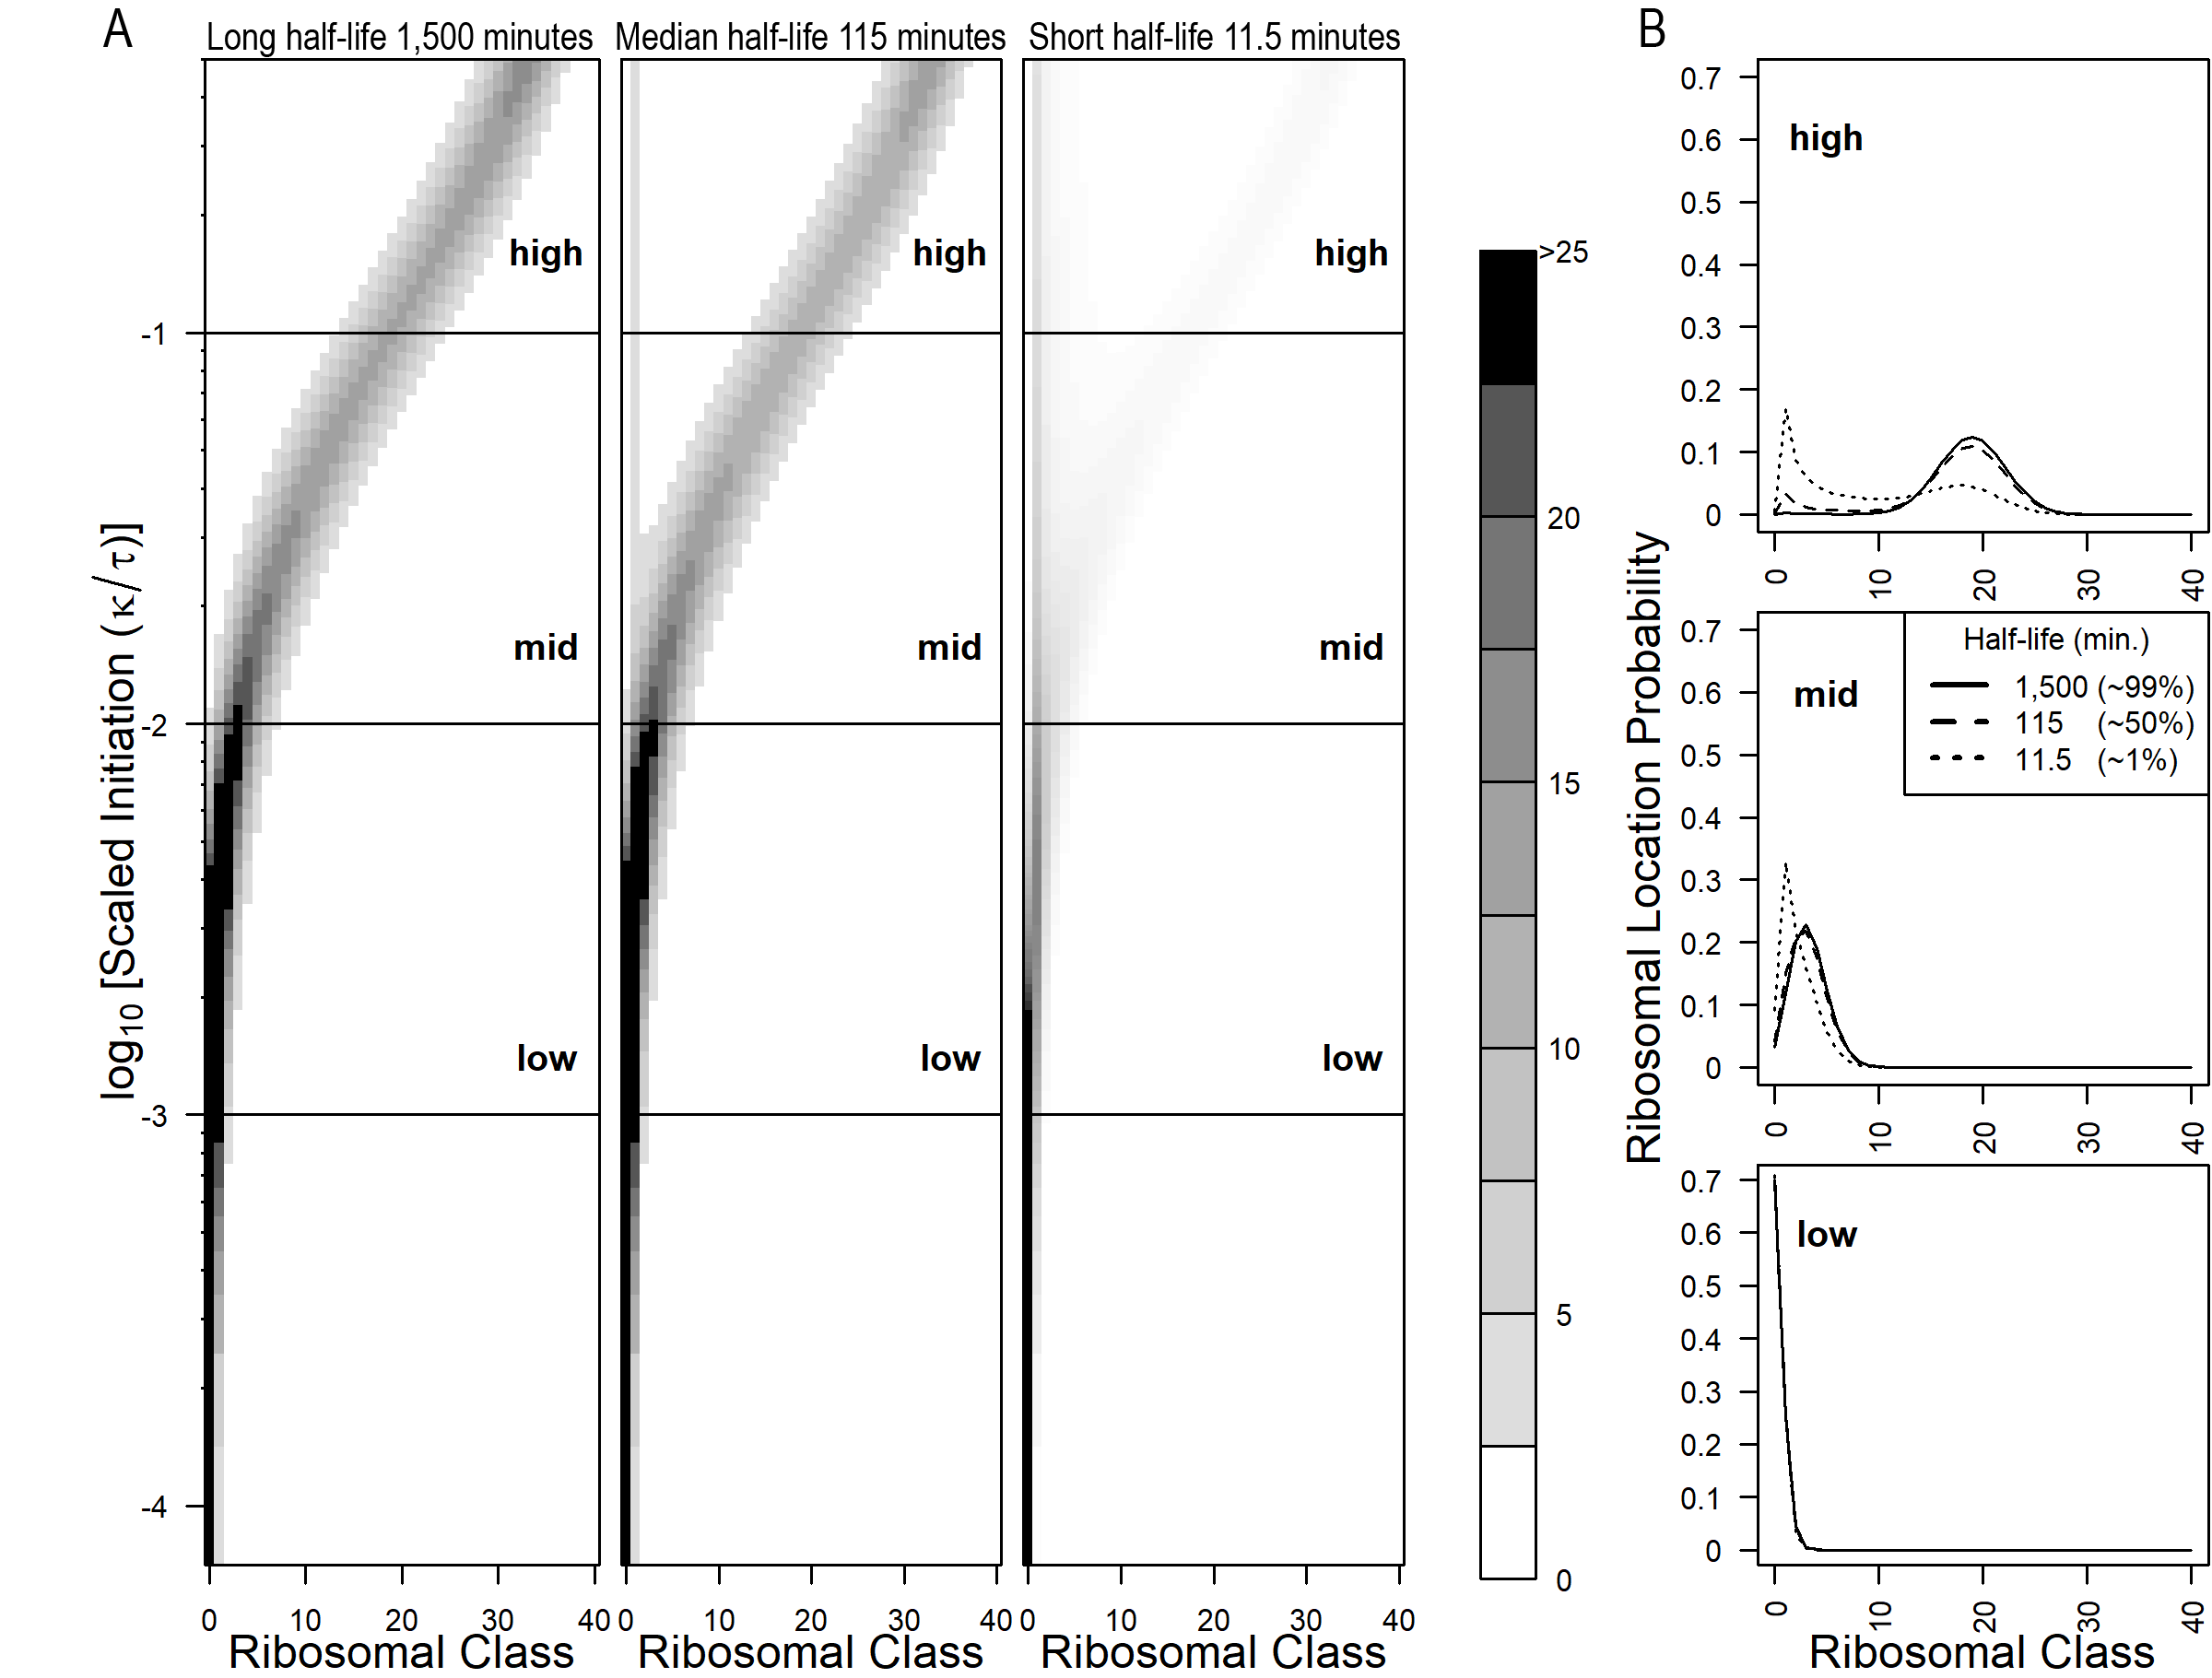
\includegraphics[width=140mm]{Images/2023-07-09_Figure2_At_Marking_Rate_range_medianlength_with_labels.png}
\caption{{\bf Low decapping rates $\mu$ in Arabidopsis result in polysome class distributions centered at higher $i$ and more mRNA abundance in the capped vs decapped polysome classes.} {\bf  A)}  Heatmaps for the full model. Left) low $\mu$ ($7.7\times 10^{-6}$ /s) Center) median $\mu$ (1$\times 10^{-4}$ /s) Right) $\mu$ ($1\times 10^{-3}$ /s) {\bf B)} individual density profiles for low (0.001), mid (0.01) and high (0.1) scaled initiation values for each $\mu$. All results calculate with \imax = 41.}
%\centering Red: decapped class, Green: capped class, Blue: Total= capped+decapped classes}
\label{fig7}
\end{center}
\end{figure*}



\subsection*{Decapping rate and ribosomal load determine ratio between capped and decapped states}
 As shown in previous results, higher decapping rates $\mu$ lead to lower \MRL in the capped state and increase mRNA abundance in the decapped state.
Using eq. (\ref{eq:odds}), we can determine how much of the mRNA population is in the capped state.
We produced output across all scaled initiation values $\kappa'$ and under the 1\textsuperscript{st}, 50\textsuperscript{th} and 99\textsuperscript{th} percentiles for decapping rates in both yeast and Arabidopsis (Fig \ref{fig8}). 
We note two patterns. First as the $\kappa'$ increases, so does the amount of mRNA in the decapped class  \mvechatstar increases. 
Secondly and similarly, higher $\mu$ shifts mRNA population from the capped state to the decapped state as previously seen in Fig \ref{fig6} and \ref{fig7}.  


\begin{figure}[!h]
\begin{center}
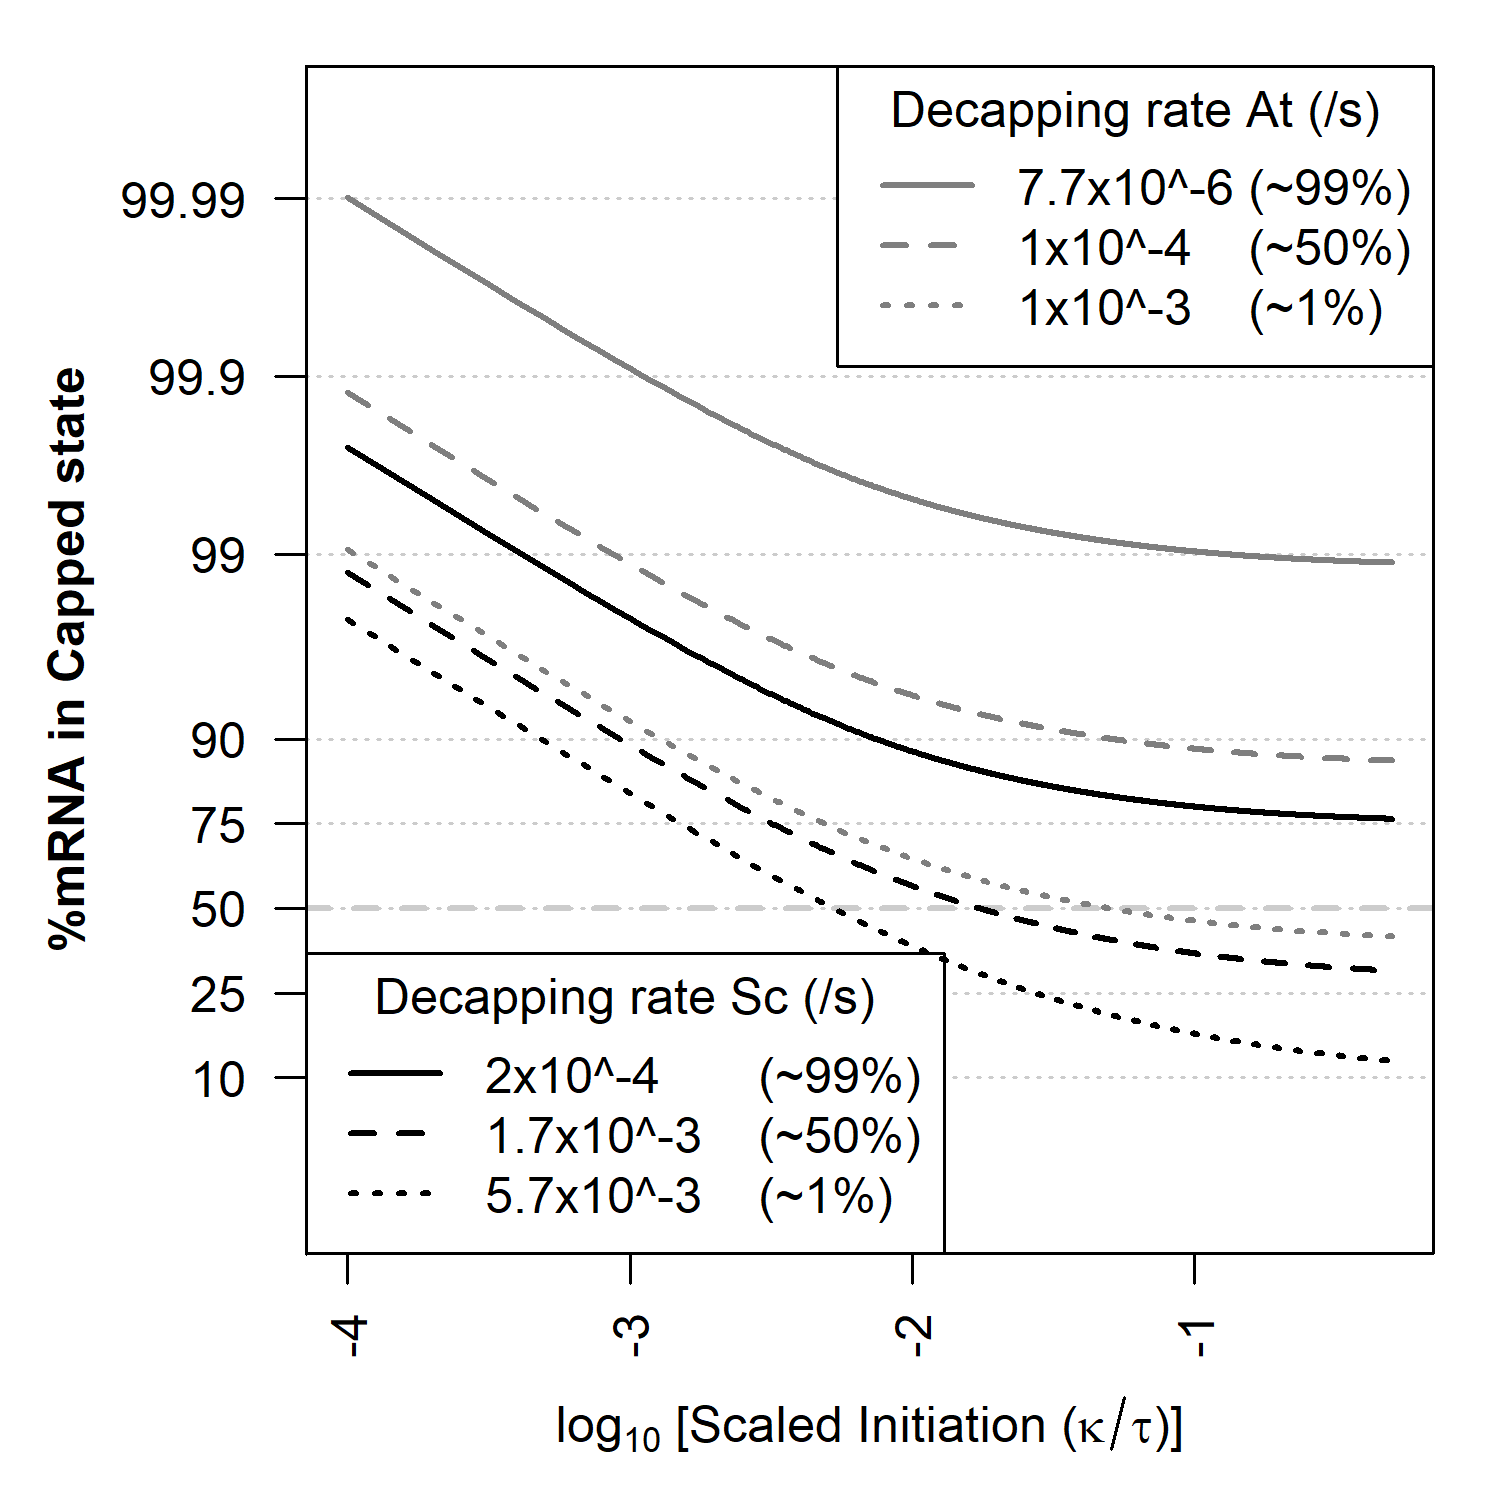
\includegraphics[width=70mm]{Images/2023-07-28_logodds.png}
\caption{{\bf Percentage of mRNA in the capped state for a range of decapping rates in yeast} ( low $\mu$ ($2\times 10^{-4}$ /s), median $\mu$ ($1.7\times 10^{-3}$ /s), high $\mu$ ($5.7\times 10^{-3}$ /s)) and Arabidopsis( low $\mu$ ($7.7\times 10^{-6}$ /s, median $\mu$ (1$\times 10^{-4}$ /s), high $\mu$ ($1\times 10^{-3}$ /s)). }
%\centering Red: decapped class, Green: capped class, Blue: Total= capped+decapped classes}
\label{fig8}
\end{center}
\end{figure}

\subsection*{At steady state protein production is scales with coding sequence length \imax}
At steady state the \MRL increases with coding sequence length and begins to assymptote at high initiation to elongation ratio $\kappa'$ (Fig \ref{fig9}). Yet the capped state \MRL is always greater than the decapped \MRL. The \MRL of the whole system is defined by both capped and decapped \MRLs in eq. (\ref{eq:Expected_ribo_load}) as well as the transcript abundance in each state as shown in eq. (\ref{eq:System_ribo_load}).
As protein length \imax increases, mRNAs enter the decapped state at higher polysome classes. 
Therefore ribosomes take longer  to clear the mRNA, and thus increase the contribution from the decapped state. 
For $\kappa'$= 0.1, the percentage of the mRNA in the capped class is  99\% 78\%  and 35\% for \imax of 4, 39 and 194 respectively.
The \imax dependence is captured in the 1/$\tau$ term in eq. (\ref{eq:odds}).
  
\begin{figure*}[!h]
\begin{center}
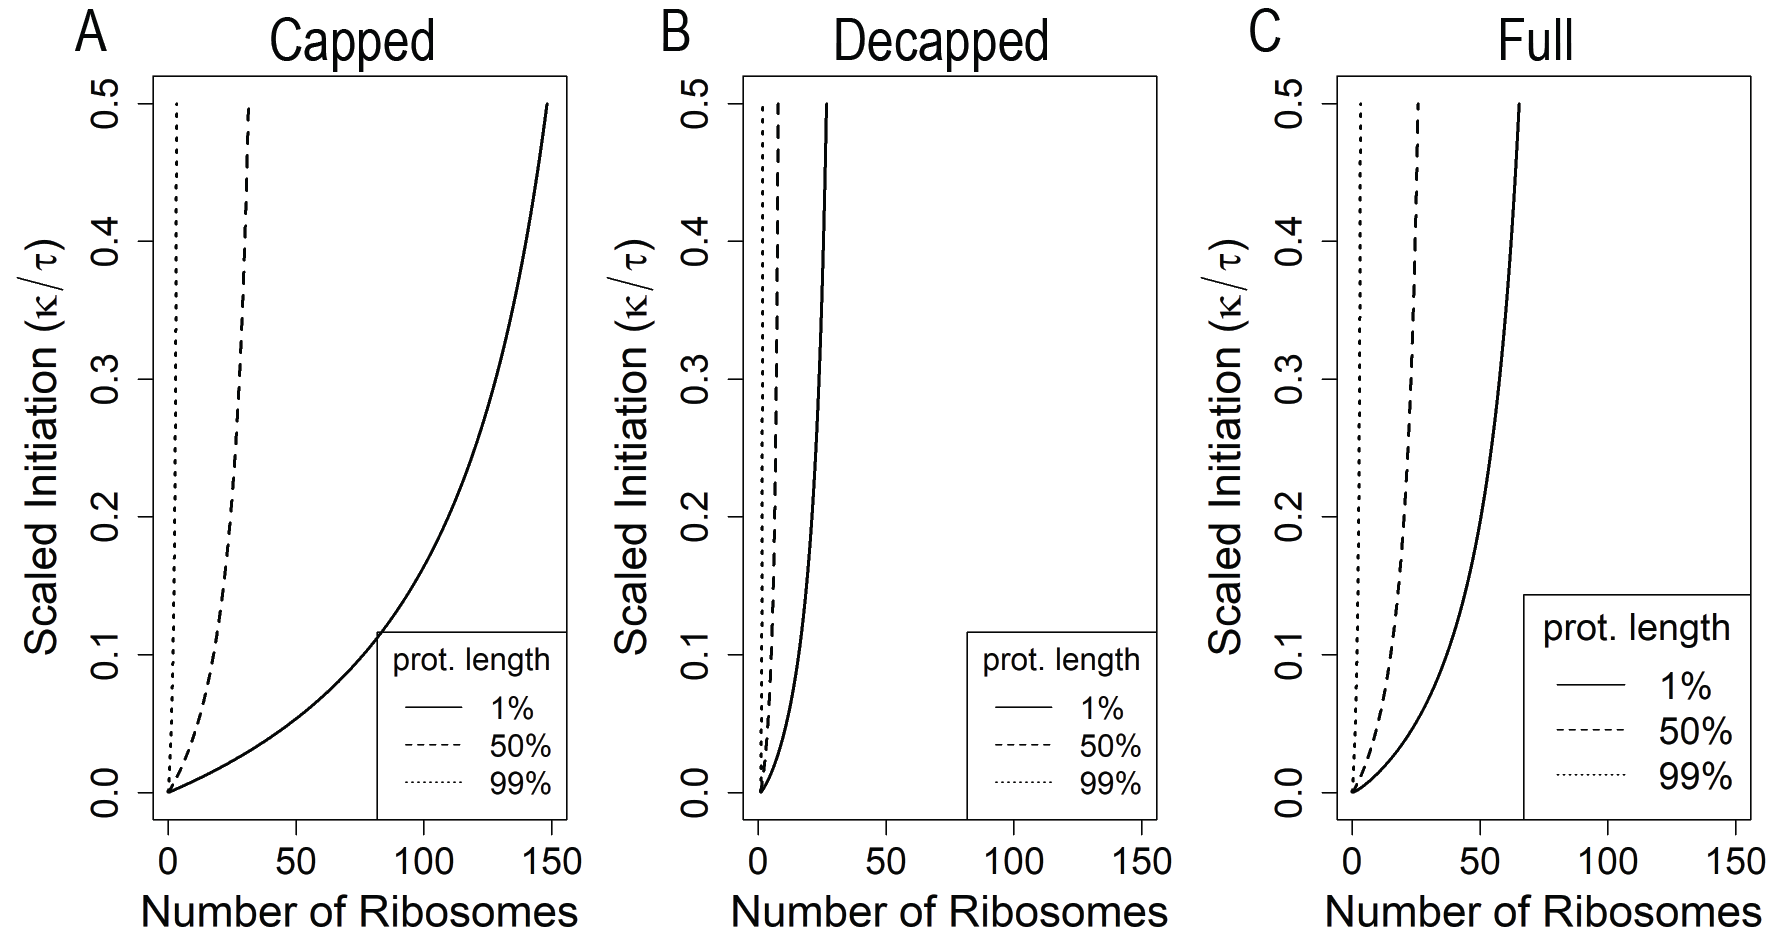
\includegraphics[width=120mm]{Images/MRL.png}
\caption{{\bf The mean ribosomal density on a transcript is dependent on coding sequence length.} 
\MRL per transcript is higher for longer transcripts. {\bf A)} Capped state {\bf B)} Decapped state {\bf C)} full model. Yeast parameters were used \imax =  4 (1\textsuperscript{st} percentile),  39 (50\textsuperscript{th} percentile), 194 (99\textsuperscript{th} percentile), low decapping rate ($2.2\times 10^{-4}$ /s), over the full scaled initiation range 0.0001- 0.5.}
%\centering Red: decapped class, Green: capped class, Blue: Total= capped+decapped classes}
\label{fig9}
\end{center}
\end{figure*}

\subsection*{Decapped state can be a significant source of protein production} 
Protein production rate (PPR) is a function of full model \MRL $\times \tau$ and plots normalized to highest possible protein output are shown in Fig \ref{fig10}.
As the decapping rate $\mu$ increases it reduces the capped and uncapped \MRL as well as shifting transcript abundance to the decapped state (Fig \ref{fig10}A).
Each of the three cases in Fig \ref{fig10} A, has been broken down into the PPR contributions from the capped and decapped states (Fig \ref{fig10}B-D). 
A surprising finding from out model is that when $\mu$ is high ($5.7\times 10^{-3}$ /s), 41\% of all protein production can arise from the decapped state (Fig \ref{fig10}D).
The reason behind this is despite the the \MRL of the decapped state being lower than the capped state as scaled initiation rises, the shift of mRNA from the capped polysome classes to the decapped polysome is enough to offset the lower $\MRL^*$

\begin{figure*}[!h]
\begin{center}
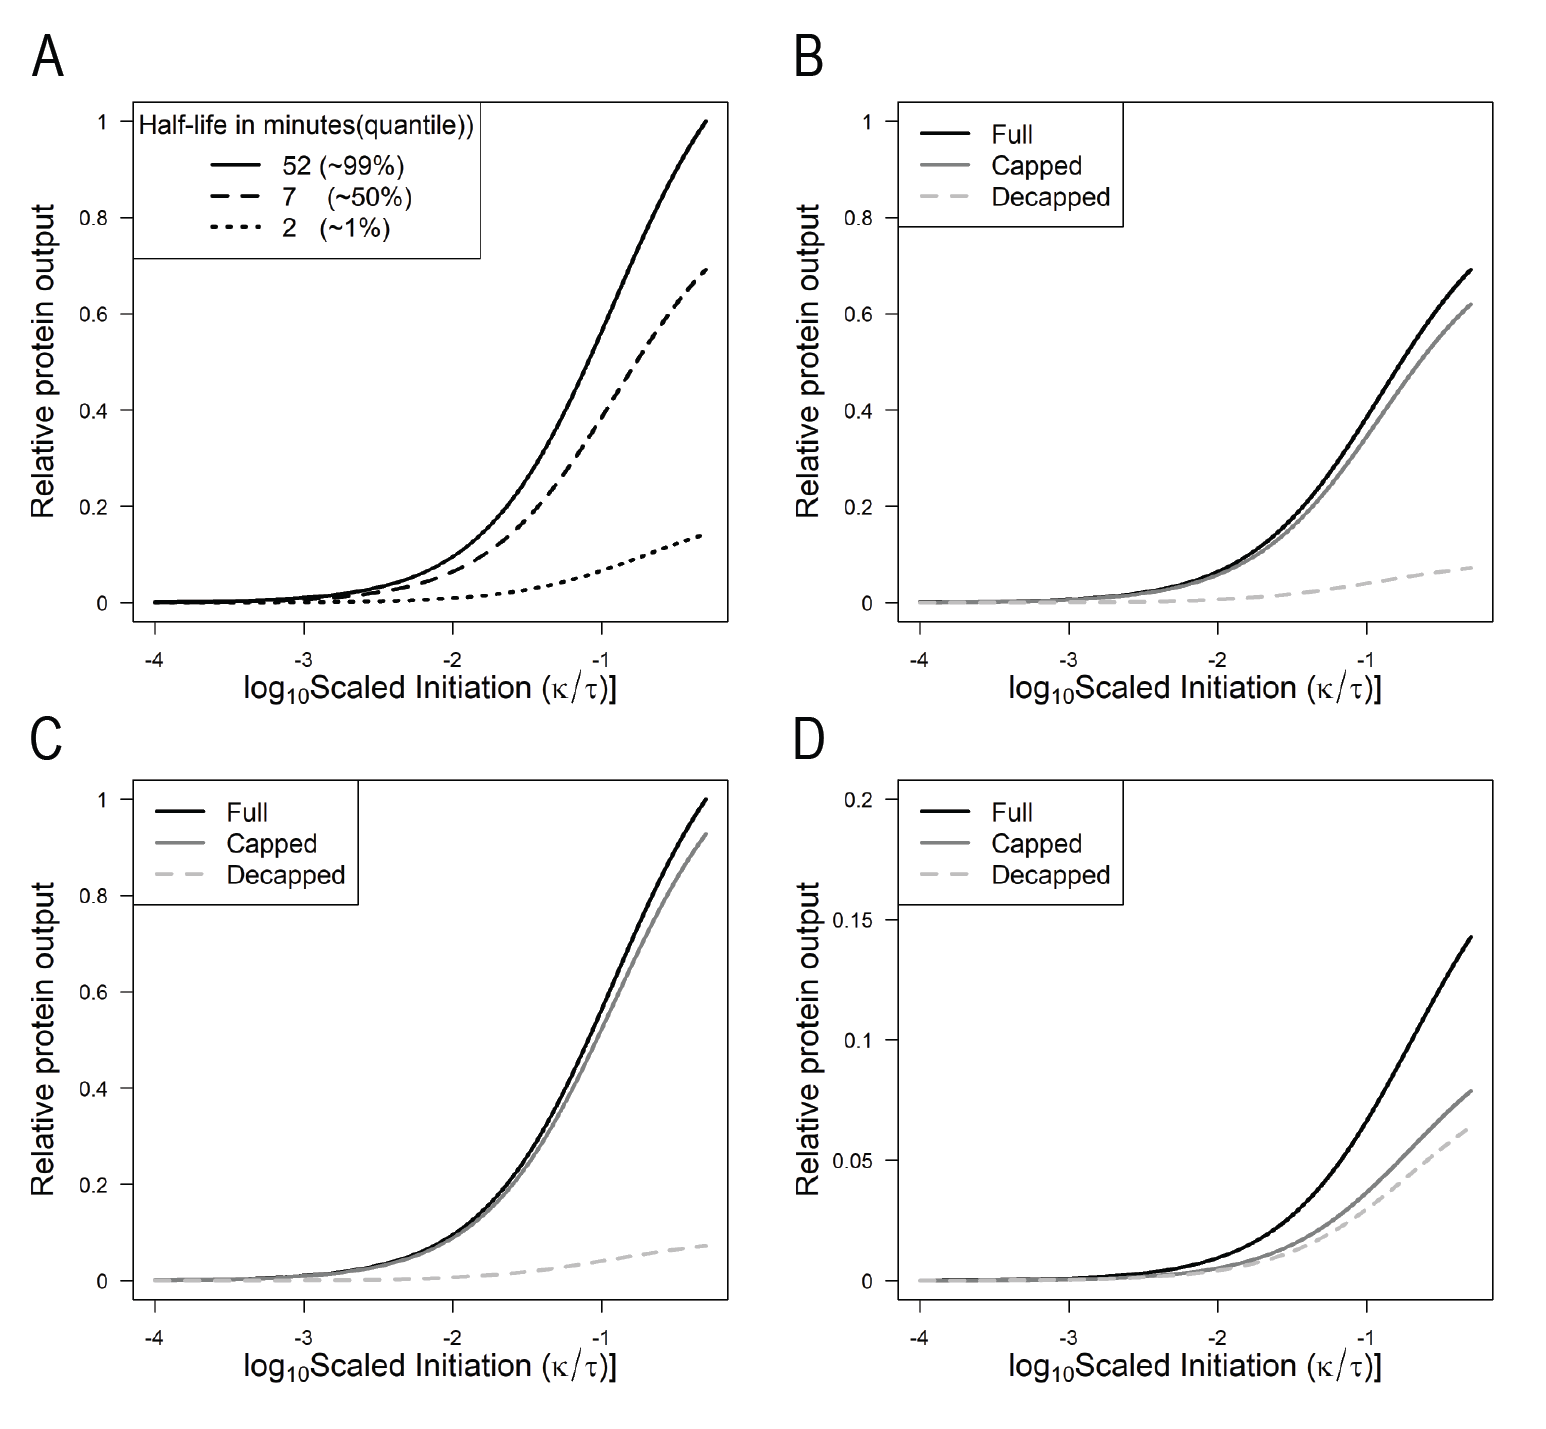
\includegraphics[width = 120mm]{Images/2023-07-17_Protein_Production_v2.png}
\caption{{\bf Estimated average protein production in yeast.} {\bf  A)} Protein production across different decapping rates  low $\mu$ ($2.2\times 10^{-4}$ /s), median $\mu$ ($1.7\times 10^{-3}$ /s), high $\mu$ ($5.7\times 10^{-3}$ /s). Total protein production is normalized to the maximal protein production across all parameters. B-D) Contribution of capped and decapped states to total protein production. {\bf B)} Low decapping {\bf C)} Medium decapping {\bf D)} High decapping. }
%\centering Red: decapped class, Green: capped class, Blue: Total= capped+decapped classes}
\label{fig10}
\end{center}
\end{figure*}


\subsection*{Model validation}

Gene specific \MRL eq. (\ref{eq:MRL}) were calculated for the genes analyzed in Duc and Song 2018 and compared to the empirical \MRL calculated from raw data from Weinberg 2016 (Fig \ref{fig11}).
Model predictions of \MRL showed a significant positive correlation to empirical \MRLs.
This result is impressive as the model performs well despite no model fitting being performed.
Model performance is further corroborated with single molecule imaging analyses.
Rescaling ribosome abundances from each single molecule study to an \imax of 39 results in loads of 1, 2.4 and 4 ribosomes from~\cite{RN30}, 3 ribosomes~\cite{RN31}, 4 ribosomes~\cite{RN32} and 1.6~\cite{RN33}.
The single molecule measurements agree with model predictions, as most transcripts have a MRL of 0-6 for median decapping rate ($1.7\times 10^{-3}$ /s) and  $\kappa' < 0.01$ and \imax of 39.
%  \item All of which align with low to mid initiation to elongation ratio \MRL predictions. 
  %\item Finally, mRNA distributions for the full model agree with signal from polysome traces (Lokdarshi 2020, Dasgupta 2023).



\begin{figure}[!h]
\begin{center}
\centering
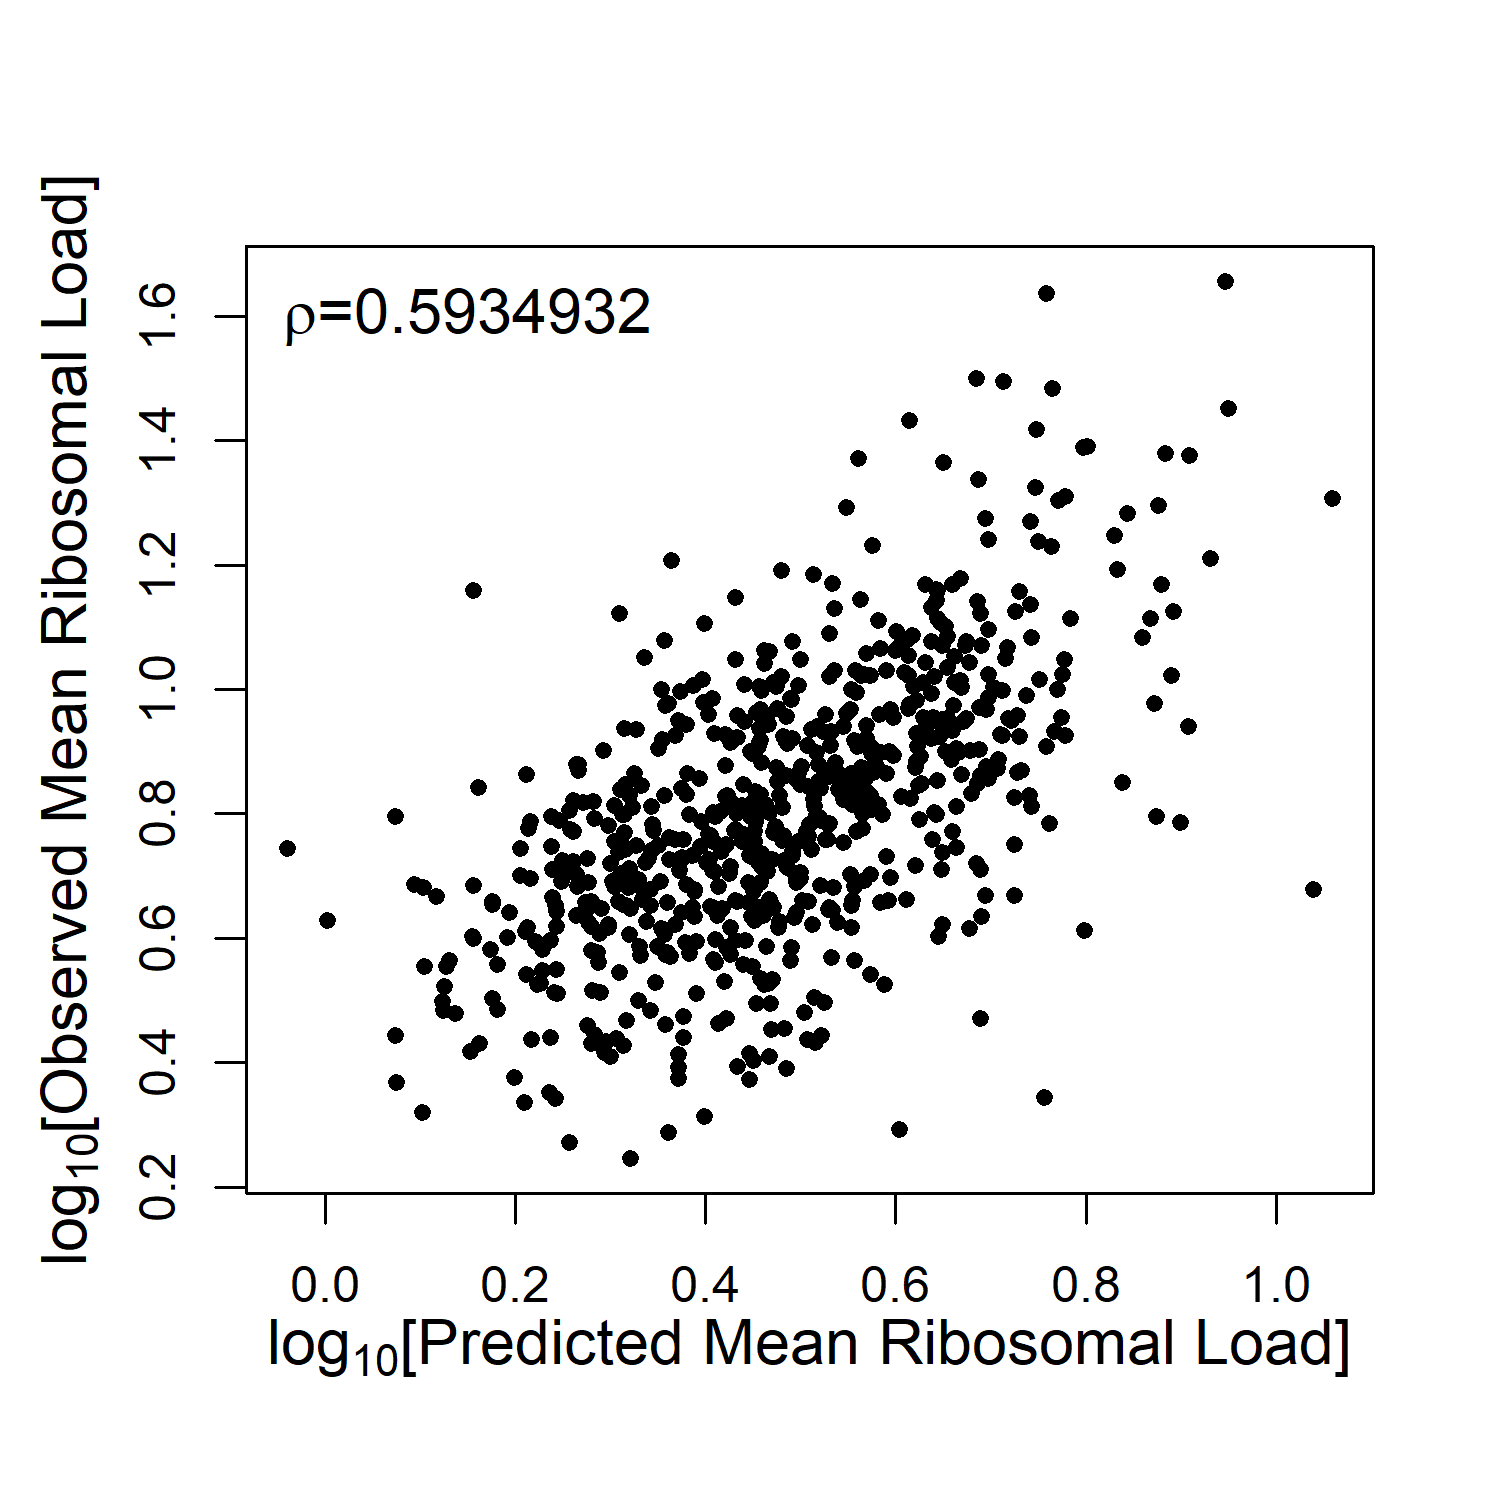
\includegraphics[width=75mm]{Images/Duc_Song_vs_model_log.png}
\caption{{\bf Predicted mean ribosomal loads coincide with observed mean ribosomal loads from Weinberg 2016.}
Using the 850 genes from Duc and song 2018, decapping rates from Presnyak 2015 were mined. Gene specific \MRL were calculated and compared to the empircal \MRL. Spearman's $\rho$ was calculated and found to be significant, pvalue $<10^{-16}$}
%\centering Red: decapped class, Green: capped class, Blue: Total= capped+decapped classes}
\label{fig11}
\end{center}
\end{figure}



\section*{Discussion}

In this study we develop, analyze, and validate a novel coupled ODE model of mRNA polysome classes %\mmpar{Terminology: do we like `mRNA polysome populations'?}\rmpar{Yes}
which includes the contributions of mRNA transcription, the initiation, elongation (implicitly), and termination of translation as well as mRNA degradation through 5' decapping and cotranslational decay.

\subsection*{Model Formulation \& Structure}

Although our model is only a very simplified description of the mRNA polysome population and, in turn, protein translation, it studies the underexplored interaction of protein translation with the process of mRNA degradation~\cite{RN11}. The process of translation is dependent on the underlying population of capped, translationally competent mRNAs. However, empirical measurements suggest that $\sim 12\%$ of transcripts are undergoing co-translational decay~\cite{RN4}. To undergo co-translational decay, the 5' cap has to removed and exonucleases trail behind the last loaded ribosome on a transcript, processing codons as they exit behind the ribosome. 5' decapping is a common pathway in many organisms and accounts for decay; for example $\sim 68\%$ of Arabadopsis genes are preferentially degraded through 5' degradation~\cite{RN28}.
%  \mmpar{I uncommented this point, can you reconcile it with the previous sentence? \textbf{R:} Done. The first is a statement of the proportion of the population undergoing decay. The second the proportion of the genome that preferentially uses this pathway for decay.} 
Our model includes 5' mRNA decapping followed by cotranslational decay, permiting the analysis of the decapped mRNA state (called degratome in~\cite{RN34}), changes in mean number of ribosomes per transcript \MRL for capped and decapped states and the contribution of cotranslational decay to protein production.

In addition to being more biologically realistic, structuring the mRNA population by its polysome classes (ribosome load) and the status of its 5' cap allows us to understand how the the rates mRNA production $\lambda$, decapping $\mu$, protein elongation $\tau$, and the clearance rate $\delta$ of decapped and ribosome free mRNAs $\mhatstar_0$ shape the steady state distribution of a gene's mRNA population across polysome classes and capping state (Fig \ref{fig3}-\ref{fig5}).

Analytical and numerical solutions show transcription rate $\lambda$ acts as a scaling factor such that the abundances of all of the mRNA polysome classes are proportional to $\lambda$.
 In other words, the total abundance of the capped and decapped mRNA polysome classes $\mvechat$ and $\mvechatstar$ are simply proportional to $\lambda$ (see (\ref{eq:capped_sum}) where $\sum_{i = 0} ^\imax m_i = \lambda/\mu$ and (\ref{eq: marked_total_pop}), respectively).
  The fact that the abundance of the entire capped and decapped mRNA polysome classes are proportional to the transcrption rate $\lambda$ is consistent with intuition, as $\lambda$ increases, so does the abundance of both the capped and decapped populations.
  Similarly, the fact that the abundance of the capped mRNA polysome classes declines as an inverse function of the decapping rate $\mu$ is also consistent with intuition.
  Because it is the ratio of $\lambda$ and $\mu$, rather than their individual values, that determine the size of the capped mRNA polysome classes, our model indicates that there will be an infinite set of transcription $\lambda$ and decapping rates $\mu$ that can result in the same population size of capped mRNA polysomes.
  All else being equal, this result suggests that these rates could vary greatly between genes with similar abundances.


The fact that changes in the mRNA transcription rate  $\lambda$ only scales, rather than shapes, the relative distribution of mRNA polysome classes allows us to turn our focus to how the remaining model parameters, $\kappaprime = \kappa/\tau$, $\mu$, and $\delta$ alter the \emph{relative} distribution of the capped and decapped mRNA polysome classes \mvechat and \mvechatstar, respectively.

For example, focusing on the relative distribution of the capped mRNA polysome classes $\mvechat$, our model indicates that it is the ratio of scaled translation initiation $\kappaprime = \kappa/\tau$ to decapping $\mu$ which determines the distribution \mvechat, and thus its mean ribosome load  (Fig \ref{fig3}).
    Additionally, when the initiation rate is much less than the decapping rate $\kappaprime/\mu \ll 1$, the distribution of capped mRNA polysome classes $\mvechat$ is greatest in the ribosome free polysome class $i=0$ and declines rapidly with with ribosome load $i$.
    As $\kappaprime/\mu$ increases, the distribution of capped mRNA polysome classes shifts away from the lower bound of $i = 0$ appears to follow a truncated gaussian distribution.
    In contrast, it is only at very high and generally unrealistic values of $\kappaprime/\mu$ (i.e.  when $\kappa>>\mu or \tau$, so that $\kappaprime/\mu > 10$) do we see the peak of the distribution of capped mRNA polysome classes approach $\imax$.



Shifting our focus to the relative distribution of the decapped mRNA polysome classes \mvechatstar, our model provides a number of important insights .
Surprisingly, in the special case of the decapped, ribosome free mRNA class $\mhat_0^*$, we find its abundance is decoupled from the dynamics of the rest of the population.
  This decoupling has a number of important implications.
  For example, the steady state abundance of $\mhat_0^* = \lambda/\delta$ and, thus, depends only on the ratio of the mRNA transcription rate $\lambda$ to the mRNA clearance rate $\delta$ (equation \ref{eq:decapped_solution}).
  If the transcription rate $\lambda$ of new, capped, but ribosome free mRNAs $\mhat_0$ is substantially lower than the per capita mRNA clearance rate of decapped, ribosome free mRNAs $\delta$, such that  $\lambda \ll \delta$, then our model predicts that there will be few mRNAs in the $\mhat_0^*$ class ($\mhat_0^* \ll 1$).
  Because $\mhat^*_0$ has no impact on the rest of the mRNA population, this result allows us to greatly simplify our analysis further since we need not consider $\mhat_0^*$ nor the parameter $\delta$.

Focusing now on the steady state abundance of the ribosome occupied decapped mRNA polysome classes, i.e.  $\mhat_i^*$ where $i > 0$, we find that the distribution of $\mhat^*_i$  depends on the gene specific ribosome elongation rate $\tau$ (where `elongation`  includes the ribosome's reading of the mRNA's stop codon) and the distribution of capped mRNA $\mhat_i$ (Fig \ref{fig4}).
\label{item:protein_production} This finding implies that because the density of $\mhat^*_i$ monotonically decreases with $i$, the distribution of decapped mRNA polysome classes is skewed and dominated by lower polysomal classes.
  This is monotonic decline coupled with the fact that the decapped ribosome free polysome class $\mhat_0$ does not contribute to protein production, implies that \MRL of the decapped mRNA polysomes must be less than \MRL the of the capped mRNA polysomes.
  Thus, while the decapped class does contribute to protein production, substantially under low decapping ($\mu> 5.7 \times 10^{-3}$) or large \imax, its contributution to the mRNA population's protein production will always be less than  $50\%$.



The full model combines the distributions of the capped and decapped states and is equivalent to mRNA population that is often measured in translational assays.
The full model distribution is strictly unimodal when initiation occurs and $\kappaprime/\mu \ll 1$ (Fig \ref{fig6} and \ref{fig7}) and the majority of transcripts are in the capped state ($\sum \mvechat >> \sum \mvechatstar$), effectively .
The distribution is also unimodal when the $\kappaprime << 0.01$, meaning that the \MRL is low and near the $i=0$ bound. 
In all other cases the distribution of polysome classes is bimodal. The high peak arises from the capped state, while the small novel  peak comes from the decapped states. 
To the best of our knowledge, the only prior model that combines cotranslational decay and translation, agrees with our findings of decreased \MRL when decapping occurs~\cite{RN22}. However, they didn't explore a range of biologically relevant parameters nor did they analyze the contributions from the capped and decapped polysome classes separately.

The model formalizes the interplay between mRNA decapping $\mu$ and initiation elongation ratio $\kappa/\tau$ and its effect on protein production.
By using eq.  [\ref{eq:System_ribo_load}] we can estimate protein production rate.
Shifts in mRNA between capped and decapped states as well as changes in \MRL control protein production.
As expected, increasing $\mu$ raises the proportion of decapped transcripts \mvechatstar compared to capped transcripts \mvechat.
Increasing ratio of initiation to elongation rates $\kappa/\tau$ also results in an increase of decapped mRNAs \mvechatstar.
As $\kappa/\tau$ increases the \MRL of the capped population \mvechat increases, transcripts enter the decapped state at higher polysomal classes and thus take longer to reach $m_0^*$.
At high $\mu$ this shift in transcripts is enough to shift more protein production to the decapped polysome classes, but not enough to overtake the capped protein production.
One final consideration is the assumption that the mRNA clearance rate $\delta >> \lambda$, and therefore $\mhatstar_0$ will be negligible and won't affect protein production at the population scale. If $\mhatstar_0$ is small our current results act as an upper bound of the protein production contribution from the decapped class. 


A unique property of our model is that it can differentiate the capped and decapped states individual contributions to protein production. 
A surprising prediction from our model is that genes with  high decapping rates (e.g. $\mu  \sim 5 \times 10^{-3}$ or a half-life of $\sim 120 \sec$) has almost (but never more than) half of its protein production coming from the decapped mRNA polysome classes (Fig \ref{fig10}).
The high protein production from the decapped polysome classes suggests that mRNAs with high decapping rate can produce more protein than would be expected based on this $M_{tot} = \frac{\lambda}{\mu}$ alone. 


\subsection*{Model Validation}

In addition to studying the general behavior of our model, we validate this behavior using empirically based parameter values.
In general, we find that our model's predictions of mRNA distributions, when parametrized with biologically relevant values, are highly consistent with a wide range of empirical data.
For example, we predicted \MRL using empirical values for initiation to elongation rates ratio $\kappa'$~\cite{RN13} and decapping rate $\mu$~\cite{RN27} and compared them to the empirical \MRL from~\cite{RN29} and found a strong correlation despite having performed no additional model fitting. This supports the idea that the model is a useful representation of the complex processes underlying protein production.

The $\kappa'$ estimates utilized are only for highly translated genes (16\% of alll detected genes), and most others would fall in a range of $\kappa'<0.01$~\cite{RN13}.
Taking the overall low $\kappa'$ values, our model predicts that a median length protein of \imax =39 (351aa) would have 10 or fewer ribosomes loaded, which agree with the predominance of low polysomes (<10) seen polysome gradient traces~\cite{RN35, RN36}. 
By the same logic, we find that single molecule measurements of translation~\cite{RN30,RN32,RN33,RN31} (Morisaki 2016, Yan 2016, Wang 2016, Wu 2016, Section 3.6) all fall in the same low polysome range.
Finally, the fraction of mRNA predicted in the capped and decapped class  are consistent with population wide estimates (\cite{RN4}, Fig \ref{fig10}). 


\subsection*{Model limitations, extensions and future work}

Our model's assumptions about the process of mRNA decapping, the continued translational competence of transcript ribosomes bound prior to decapping, and degradation of mRNA solely from the decapped and ribosome free class $m_0^*$  closely resembles the biological process of co-translational mRNA decay. While the existence of co-translational mRNA decay is well established~\cite{RN4,RN28}, other mechanisms exist with different outcomes for translation. 3' decay prevents bound ribosomes from completing translation and would send all transcripts into the $m_0^*$ class . Mechanisms utilizing endonucleolytic decay due to no go decay or nonsense mediated decay would potentially allow ribosomes downstream of the cleavage site to terminate but not those upstream~\cite{RN38,RN2}. Thus,  the site of the endonucleolytic decay a transcript in $m_i$ would end up in $m_{j^*}$, where $j < i$.

Currently there is debate about the contributions of the protective effects of ribosome association vs. ribosome stalling to mRNA transcript stability.
While our model currently does not include the protective effects of translation or stall prone codons, it should be possible to do so.
The protective effects of ribosomal loading which could be modeled by making the decapping rate $\mu $ a function of $i$, e.g. $(1-i/\imax)$. Otherwise one could have a higher decapping rate for $m_0$ and a lower decapping rate for the other polysomal classes.
The protective effects of translation on decapping could increase per ribosome, but eventually at high \MRL could trigger ribosome associated decay pathways through ribosomal collisions, so $\mu$ would be a non monotonic function of $i$. This would require analysis on an individual transcript basis.
Our model does not consider codon specific effects such as pausing sites, difficult to fold regions of a protein or codon usage, or protein quality control~\cite{RN39}.
Pausing sites could be addressed by splitting each polysome class into two regions and could approximate a ribosome flow model of only two regions, a 5' and 3', split by the pausing site. Current models of translation focus mainly on the behavior of the average transcripts. However this ignores the changing population of mRNAs necessary for protein production. 
Developing a more quantitative understanding of how different factors affect a gene's mRNA stability and, in turn, protein expression, relevant to a wide range of applied molecular biology (e.g. the design of efficient heterologous genes expression and mRNA vaccines)~\cite{RN40}.



%
%
% 
%
%
%\section*{Supplementary Text}
%
%%%%%%%%%%%%%%
%In this section we present the matrix vector formulation of the model used to obtain both the analytical and numerical solutions in the main text. Additionally, we describe the analytical solution to the capped system. 
%%Note that from here forward the capped and decapped subsystems are presented separately, the benefits of taking this approach will become evident as we proceed.  
%
%
%\subsection*{Matrix-vector Formulation of ODE System}
%It is frequently useful to work with the matrix-vector formulation for a system of ODE.
%In this model, the dynamics of the decapped and capped mRNAs can be represented as,
%\begin{equation}
%\vec{M}'=\boldsymbol{F}\vec{M}+\vec{B},
%\end{equation} 
%where $\vec{M}\in\mathbb{R}^{2(\imax+1)}$ is a vector of all state variables, ordered here as $m_0$, $m_1$, ..., $m_{\imax}$, $m^*_0$, $m^*_1$, ..., $m^*_{\imax}$, $\vec{M}'$ is the vector containing the first derivatives of $\vec{M}$ with respect to time, $\bs{F}\in\mathbb{R}^{2(\imax+1)\times 2(\imax+1)}$ is the matrix representing the full model (Equation\ref{eq:full_matrix}), and $\vec{B}\in\mathbb{R}^{2(\imax+1)}$ is the vector of $\lambda$ as the first component and 0s else.
%Using the functional forms presented above, matrix formulations are provided next.
%
%As opposed to explicitly listing elements of the full model matrix-vector representation we found that it is more convenient to utilize the block structure that emerges in this system and explicitly provide the block components.
%The matrix $\bs{F}$ is block lower-diagonal and is given in Equation\ref{eq:full_matrix}.
%\begin{equation}
%\bs{F}=\left(\begin{array}{cc}
%\bs{U} & \bs{0} \\
%\bs{\mu} & \bs{R}
%\end{array} \right).
%\label{eq:full_matrix}
%\end{equation}
%The upper-left block, $\bs{U}$, corresponds to the capped state variables, where $\bs{U}$'s general form is provided in Equation\ref{eq:capped_matrix}.
%The upper-right block is a matrix of all zeros, $\bs{0}\in\mathbb{R}^{\imax+1\times \imax+1}$.
%Using $\bs{I}$ to represent the $\imax+1\times \imax+1$ identity matrix, the lower-left block is $\bs{\mu}=\mu_0\bs{I}$, a diagonal matrix with the constant $\mu_0$ on the diagonal and 0s else.
%The lower-right block, $\bs{R}$, corresponds to the decapped state variables and its form is provided in Equation\ref{eq:decapped_matrix}.
%
%The matrix $\bs{U}$ is $(\imax+1\times \imax+1)$ dimensional and is tri-diagonal with non-zero entries on the diagonal, super-, and sub-diagonals,
%%\pagebreak
%\begin{strip}
%\begin{adjustwidth}{-2.25in}{0in} 
%\begin{equation}
%\bs{U}=\left(\begin{array}{cccccc}
%-(\kappa_0+\mu_0) & \tau_0\frac{1}{\imax} &  &  &  & \\
%\kappa_0 & \left(1-\frac{1}{\imax} \kappa_0+\mu_0+\tau_0\frac{1}{\imax}\right) & \tau_0\frac{2}{\imax} &  &  & \\
%   &\ddots        & \ddots        & \ddots & &  \\
%   & &    1-\frac{(i-1)}{\imax}\kappa_0 & -\left(1-\frac{i}{\imax}\kappa_0+\mu_0+\tau_0\frac{i}{\imax}\right) & \tau_0\frac{i+1}{\imax} & \\
%                  &         &        & \ddots  & \ddots & \ddots \\
%     
%                          &        &  &  & \frac{1}{\imax}\kappa_0 & -\left(\mu_0+\tau_0\frac{\imax}{\imax}\right)
%\end{array}\right).
%\end{equation}
%
%In the representation given in Equation\ref{eq:capped_matrix}, all blank entries are 0.
%The $(\imax-1)^{\text{th}}$ row has been suppressed in Equation\ref{eq:capped_matrix}, but it can be generated using the formula included for the $i^{th}$ row.
%
%The matrix $\bs{R}$ is the lower-right block in the block lower-diagonal matrix $\bs{F}$ (Equation\ref{eq:full_matrix}),
%\begin{equation}
%\bs{R}=\left(
%\begin{array}{ccccccc}
%-\delta & \tau_0\frac{`}{\imax} & & & & & \\
% & -\tau_0\frac{1}{\imax} & \tau_0\frac{2}{\imax} & & & &\\
% & & \ddots & \ddots & & & \\
% & & & -\tau_0\frac{i-1}{\imax} & \tau_0\frac{(i+1)}{\imax} & & \\
% & & & & \ddots & \ddots & \\
% & & & & & -\tau_0\frac{(\imax-2)}{\imax} & \tau_0\frac{\imax}{\imax} \\
% & & & & & & -\tau_0\frac{\imax}{\imax}
%\end{array}
%\right),
%\end{equation}
%\end{adjustwidth}
%\end{strip}
%$\bs{R}$ is upper-diagonal with only non-zero entries on the diagonal and the super-diagonal.
%
%\subsubsection*{Capped Subsystem Matrix-vector Representation}
%As a group the capped subsystem decouples from the decapped subsystem, as such the capped subsystem can be solved independently of the decapped subsystem.  
%The matrix-vector formula representing the capped subsystem is \begin{equation}
%\vec{m}'=\bs{U}\vec{m}+\vec{b},\end{equation} where $\vec{m}\in\mathbb{R}^{\imax+1}$ is the vector of capped state variables ordered $m_0$, ..., $m_{\imax}$, $\vec{m}'$ is the vector containing the first derivatives of $\vec{m}$ with respect to time, $\bs{U}\in\mathbb{R}^{\imax+1\times \imax+1}$ is the matrix representing the capped subsystem (\ref{eq:capped_matrix}), and $\vec{b}\in\mathbb{R}^{\imax+1}$ is the vector of $\lambda$ as the first component and 0s else.
%With all equations defined for the full ODE system, include matrix-vector representations, the next section outlines methods for finding steady-state solutions to the system.
%
%
%\subsubsection*{Capped state steady state solution}
%
%The capped system can be split into two components: Total transcripts in the capped state and how the transcripts are distributed across polysome classes. 
%From manual exploration of model solutions of the capped state at low \imax values. 
%We discovered that the capped class transcript number is determined by $\lambda/ \mu$
%	
%The solution to the system, as presented previously, can be expressed in the determinant-adjoint form:
%	\begin{equation*}
%		\vec{m}=-\frac{1}{\det[\bs{U}]}Adj[\bs{U}]\vec{b}.
%	\end{equation*}
%As $\vec{b}$ is [$\lambda$ 0 0 0 ... 0]. Only the first column of the adjoint matrix contributes to the result. 
%	\begin{equation*}
%		Adj[\bs{U}]\vec{b} = \lambda\vec{a}
%	\end{equation*}	
%and
%	\begin{equation*}
%		\sum_{j=0}^{\imax}\vec{a}_j = a_{tot} 
%	\end{equation*}
%With this we can factor our solution into two parts: 1) the total transcript abundance and 2) The distribution of transcript across the polysome classes.
%	\begin{equation*}
%		\vec{m}=-\frac{\lambda a_{tot}}{\det[\bs{U}]} \frac{\vec{a}}{a_{tot}} 
%	\end{equation*}
%Where:
%	\begin{equation*}
%		\frac{\vec{a}}{a_{tot}} = \vec{p}_m
%	\end{equation*}
%The vector $\vec{p}_m$ sums to one and contains the probabilities of finding and mRNA in each class in the capped state. Now we are left with
%	\begin{equation*}
%		\vec{m}=-\frac{a_{tot}}{\det[\bs{U}]} \: \lambda\vec{p}_m
%	\end{equation*}
%If we sum across all classes to get the total mRNA population we find,
%	\begin{equation*}
%		\sum_{i=0}^{\imax}m_{i} =-\sum_{i=0}^{\imax} \frac{a_{tot}}{\det[\bs{U}]} \: \lambda\vec{p}_m =-\frac{a_{tot}}{\det[\bs{U}]} \: \lambda = \frac{\lambda}{\mu}
%	\end{equation*}
%	\begin{equation*}
%		-\frac{a_{tot}}{\det[\bs{U}]} = \frac{1}{\mu}
%	\end{equation*}
%We finally arrive at,
%	\begin{equation} 
%		\vec{m}=\frac{\lambda}{\mu}\vec{p}_m
%	\end{equation}
%
%
%The terms on the left hand side of the equation represent the total transcript population. The right hand side is the vector of probabilities, one entry for each class and is a function of $\kappa$, $\tau$, and $\mu$.	
%

\begin{thebibliography}{10}

\bibitem{RN21}
Ashworth W, Stoney PN, Yamamoto T.
\newblock {States of decay: The systems biology of mRNA stability.}.
\newblock Current Opinion in Systems Biology. 2019;15:48-57.

\bibitem{RN8}
Bae H, Coller J.
\newblock {Codon optimality-mediated mRNA degradation: Linking translational elongation to mRNA stability}.
\newblock Mol Cell. 2022;82(8):1467-76.

\bibitem{RN1}
Browning KS, Bailey-Serres J.
\newblock {Mechanism of cytoplasmic mRNA translation}.
\newblock Arabidopsis Book. 2015;13:e0176. 

\bibitem{RN40}
Cheng F, Wang Y, Bai Y, Liang Z, Mao Q, Liu D, Wu X, Miao X.
\newblock {Research Advances on the Stability of mRNA Vaccines}.
\newblock Viruses. 2023;15(3).

\bibitem{RN3}
Collart MA, Weiss B.
\newblock {Ribosome pausing, a dangerous necessity for co-translational events}.
\newblock Nucleic Acids Res. 2020;48(3):1043-55.

\bibitem{RN26}
Cunningham F, Allen JE, Allen J, Alvarez-Jarreta J, Amode MR, Armean IM, et al.
\newblock {Ensembl 2022.}.
\newblock Nucleic Acids Res. 2022;50(D1):D988-D95.

\bibitem{RN13}
Dao Duc K, Song YS. 
\newblock {The impact of ribosomal interference, codon usage, and exit tunnel interactions on translation elongation rate variation}.
\newblock PLoS Genet. 2018;14(1):e1007166.

\bibitem{RN35}
Dasgupta A, Urquidi Camacho RA, Enganti R, Cho SK, Tucker LL, Torreverde JS, Abraham PE, von Arnim AG.
\newblock {A phosphorylation-deficient ribosomal protein eS6 is largely functional in Arabidopsis thaliana, rescuing mutant defects from global translation and gene expression to photosynthesis and growth}.
\newblock  Plant Direct. 2024;8(1):e566.

\bibitem{RN23}
Hu W, Sweet TJ, Chamnongpol S, Baker KE, Coller J.
\newblock {Co-translational mRNA decay in Saccharomyces cerevisiae}.
\newblock Nature. 2009;461(7261):225-9.

\bibitem{RN6}
Ikeuchi K, Izawa T, Inada T.
\newblock {Recent Progress on the Molecular Mechanism of Quality Controls Induced by Ribosome Stalling}.
\newblock Front Genet. 2018;9:743.

\bibitem{RN7}
Juszkiewicz S, Chandrasekaran V, Lin Z, Kraatz S, Ramakrishnan V, Hegde RS.
\newblock {ZNF598 Is a Quality Control Sensor of Collided Ribosomes}.
\newblock Mol Cell. 2018;72(3):469-81 e7.

\bibitem{RN25}
Kinsella RJ, Kahari A, Haider S, Zamora J, Proctor G, Spudich G, et al.
\newblock {Ensembl BioMarts: a hub for data retrieval across taxonomic space}.
\newblock Database (Oxford). 2011;2011:bar030. 

\bibitem{RN36}
Lokdarshi A, Guan J, Urquidi Camacho RA, Cho SK, Morgan PW, Leonard M, et al.
\newblock {Light Activates the Translational Regulatory Kinase GCN2 via Reactive Oxygen Species Emanating from the Chloroplast.}.
\newblock Plant Cell. 2020;32(4):1161-78.

\bibitem{RN34}
Ma X, Yin X, Tang Z, Ito H, Shao C, Meng Y, et al.
\newblock {The RNA degradome: a precious resource for deciphering RNA processing and regulation codes in plants}.
\newblock RNA Biol. 2020;17(9):1223-7.

\bibitem{RN9}
Medina-Munoz SG, Kushawah G, Castellano LA, Diez M, DeVore ML, Salazar MJB, et al.
\newblock {Crosstalk between codon optimality and cis-regulatory elements dictates mRNA stability}.
\newblock Genome Biol. 2021;22(1):14.

\bibitem{RN38}
Merchante C, Stepanova AN, Alonso JM.
\newblock {Translation regulation in plants: an interesting past, an exciting present and a promising future}.
\newblock Plant J. 2017;90(4):628-53.

\bibitem{RN30}
Morisaki T, Lyon K, DeLuca KF, DeLuca JG, English BP, Zhang Z, et al.
\newblock {Real-time quantification of single RNA translation dynamics in living cells}.
\newblock Science. 2016;352(6292):1425-9.

\bibitem{RN16}
Nanikashvili I, Zarai Y, Ovseevich A, Tuller T, Margaliot M.
\newblock {Networks of ribosome flow models for modeling and analyzing intracellular traffic}.
\newblock Sci Rep. 2019;9(1):1703.

\bibitem{RN4}
Pelechano V, Wei W, Steinmetz LM.
\newblock {Widespread Co-translational RNA Decay Reveals Ribosome Dynamics}.
\newblock Cell. 2015;161(6):1400-12.

\bibitem{RN27}
Presnyak V, Alhusaini N, Chen YH, Martin S, Morris N, Kline N, et al.
\newblock {Codon optimality is a major determinant of mRNA stability}.
\newblock Cell. 2015;160(6):1111-24.

\bibitem{RN15}
Reuveni S, Meilijson I, Kupiec M, Ruppin E, Tuller T.
\newblock {Genome-scale analysis of translation elongation with a ribosome flow model}.
\newblock PLoS Comput Biol. 2011;7(9):e1002127.

\bibitem{RN17}
Shah P, Ding Y, Niemczyk M, Kudla G, Plotkin JB.
\newblock {Rate-limiting steps in yeast protein translation}.
\newblock Cell. 2013;153(7):1589-601.

\bibitem{RN14}
Shaw LB, Zia RK, Lee KH. 
\newblock {Totally asymmetric exclusion process with extended objects: a model for protein synthesis}.
\newblock Phys Rev E Stat Nonlin Soft Matter Phys. 2003;68(2 Pt 1):021910. 

\bibitem{RN5}
Sieburth LE, Vincent JN.
\newblock {Beyond transcription factors: roles of mRNA decay in regulating gene expression in plants}.
\newblock  F1000Res. 2018;7.

\bibitem{RN28}
Sorenson RS, Deshotel MJ, Johnson K, Adler FR, Sieburth LE.
\newblock {Arabidopsis mRNA decay landscape arises from specialized RNA decay substrates, decapping-mediated feedback, and redundancy}.
\newblock Proc Natl Acad Sci U S A. 2018;115(7):E1485-E94.

\bibitem{RN2}
Urquidi Camacho RA, Lokdarshi A, von Arnim AG.
\newblock {Translational gene regulation in plants: A green new deal}.
\newblock Wiley Interdiscip Rev RNA. 2020;11(6):e1597.

\bibitem{RN22}
Valleriani A, Ignatova Z, Nagar A, Lipowsky R.
\newblock {Turnover of messenger RNA: Polysome statistics beyond the steady state}.
\newblock EPL. 2010;89(5).

\bibitem{RN12}
von der Haar T.
\newblock {Mathematical and Computational Modelling of Ribosomal Movement and Protein Synthesis: an overview}.
\newblock Comput Struct Biotechnol J. 2012;1:e201204002.

\bibitem{RN32}
Wang C, Han B, Zhou R, Zhuang X.
\newblock {Real-Time Imaging of Translation on Single mRNA Transcripts in Live Cells}.
\newblock Cell. 2016;165(4):990-1001.

\bibitem{RN29}
Weinberg DE, Shah P, Eichhorn SW, Hussmann JA, Plotkin JB, Bartel DP.
\newblock {Improved Ribosome-Footprint and mRNA Measurements Provide Insights into Dynamics and Regulation of Yeast Translation}.
\newblock Cell Rep. 2016;14(7):1787-99.

\bibitem{RN33}
Wu B, Eliscovich C, Yoon YJ, Singer RH.
\newblock {Translation dynamics of single mRNAs in live cells and neurons}.
\newblock Science. 2016;352(6292):1430-5.

\bibitem{RN37}
Wu J, Jaffrey SR.
\newblock {Tracking translation one mRNA at a time}.
\newblock Nat Biotechnol. 2016;34(7):723-4.

\bibitem{RN39}
Wu Q, Bazzini AA.
\newblock {Translation and mRNA Stability Control}.
\newblock Annu Rev Biochem. 2023;92:227-45.

\bibitem{RN10}
Wu Q, Medina SG, Kushawah G, DeVore ML, Castellano LA, Hand JM, et al. 
\newblock {Translation affects mRNA stability in a codon-dependent manner in human cells}.
\newblock Elife. 2019;8.

\bibitem{RN18}
Wu Q, Smith-Miles K, Zhou T, Tian T.
\newblock {Stochastic modelling of biochemical systems of multi-step reactions using a simplified two-variable model}.
\newblock BMC Syst Biol. 2013;7 Suppl 4(Suppl 4):S14.

\bibitem{RN19}
Wu Q, Tian T.
\newblock {Stochastic modeling of biochemical systems with multistep reactions using state-dependent time delay}.
\newblock Sci Rep. 2016;6:31909.

\bibitem{RN11}
Yadav V, Ullah Irshad I, Kumar H, Sharma AK.
\newblock {Quantitative Modeling of Protein Synthesis Using Ribosome Profiling Data}.
\newblock Front Mol Biosci. 2021;8:688700.

\bibitem{RN31}
Yan X, Hoek TA, Vale RD, Tanenbaum ME.
\newblock {Dynamics of Translation of Single mRNA Molecules in Vivo}.
\newblock Cell. 2016;165(4):976-89.

\bibitem{RN24}
Yates AD, Allen J, Amode RM, Azov AG, Barba M, Becerra A, et al.
\newblock {Ensembl Genomes 2022: an expanding genome resource for non-vertebrates.}.
\newblock Nucleic Acids Res. 2022;50(D1):D996-D1003.

\bibitem{RN20}
Zupanic A, Meplan C, Huguenin GV, Hesketh JE, Shanley DP.
\newblock {Modeling and gene knockdown to assess the contribution of nonsense-mediated decay, premature termination, and selenocysteine insertion to the selenoprotein hierarchy}.
\newblock RNA. 2016;22(7):1076-84.

\bibitem{RN41}
Van den Meersche K, Soetaert K, Van Oevelen D.
\newblock {An R Function for Sampling Linear Inverse Problems}.
\newblock Journal of Statistical Software, Code Snippets, 2009;30(1):1-15.
  
\bibitem{RN42}
Dowle M.
\newblock {data.table: Extension of 'data.frame'}.
\newblock R package 1.14.0 2021.

\bibitem{RN43}
R Core Team (2023)
\newblock {R: A Language and Environment for Statistical Computing}.
\newblock R Foundation for Statistical Computing, Vienna, Austria. <https://www.R-project.org/>.

\end{thebibliography}



\end{document}


